\chapter{Experimental Results and Discussion}
\label{sec:results}

We evaluate the in chapter \ref{chapter:alphalinkage} and chapter \ref{sec:beta} proposed algorithms with the in chapter \ref{chapter:datasets} discussed datasets aiming to find new subcategories for the text data and to generate better clusterings overall. The quality of the clusterings gets calculated with the in chapter \ref{chapter:costfunctions} explained cost functions.

\section{Algorithm Selection}

In general we evaluate two different types of experiments that apply for most of the datasets. Only for the synthetic dataset, we evaluate a data distribution similar to the one shown in figure \ref{fig:disksrings}.

\paragraph{Batch Data Experiments.} In the first one, we evaluate certain data batches, i.e. we subsample the $n$-th set of points in sorted order for each of the target classes. To generalize the experiments for larger datasets, we average over multiple batches. In our experiments, we evaluate all distinct combinations of $k$ classes, e.g. for multiple datasets we have 10 target classes and use 5 labels for our experiments, i.e. we evaluate all $10 \choose 5$ combinations to cover all possible subsets of the given target classes.

\paragraph{Randomized Experiments.} In the other setting, we select the points for certain classes by random. Averaging over a large number of clustering instances allows us to cover a major fraction of the dataset. To cluster a subset of the target classes, we also select the classes by random. Overall, in case both experimental settings agree, we know that the results generalize well for the underlying data distribution.

\subsection{Synthetic Data} 

Here we generate 1,000 clustering instances by random given the data distribution shown in section \ref{chapter:datasets}, i.e. all instances contain four classes, two rings and two disks. In figure \ref{fig:syntheticexperiments} we observe that all three linkage strategies perform very similarly. Only single linkage does slightly better with an error below $25\%$ while both average and complete linkage are above $25\%$. Interpolating between single and complete linkage (a) leads to significantly lower errors ($4.2\%$), where interpolating between average and complete linkage (b) does not lead to improvements. As this example motivates interpolating between single and complete linkage, we elaborate this setting further. Figure \ref{fig:syntheticexperiments} (c) shows that single linkage does very well identifying the two rings, while it tends to combine the two disk-shaped clusters in a quite early step. On the other hand, complete linkage does very well clustering the two disks, but it tends to combine the two rings (see figure \ref{fig:syntheticexperiments} (d)).

\begin{figure}[H]
\centering
\begin{minipage}{.45\textwidth}
  \centering
  \subcaptionbox{Interpolating between single and complete linkage justifies our motivation for the synthetic experiments as it reduces the error from $23.65\%$ to $4.21\%$.}
  {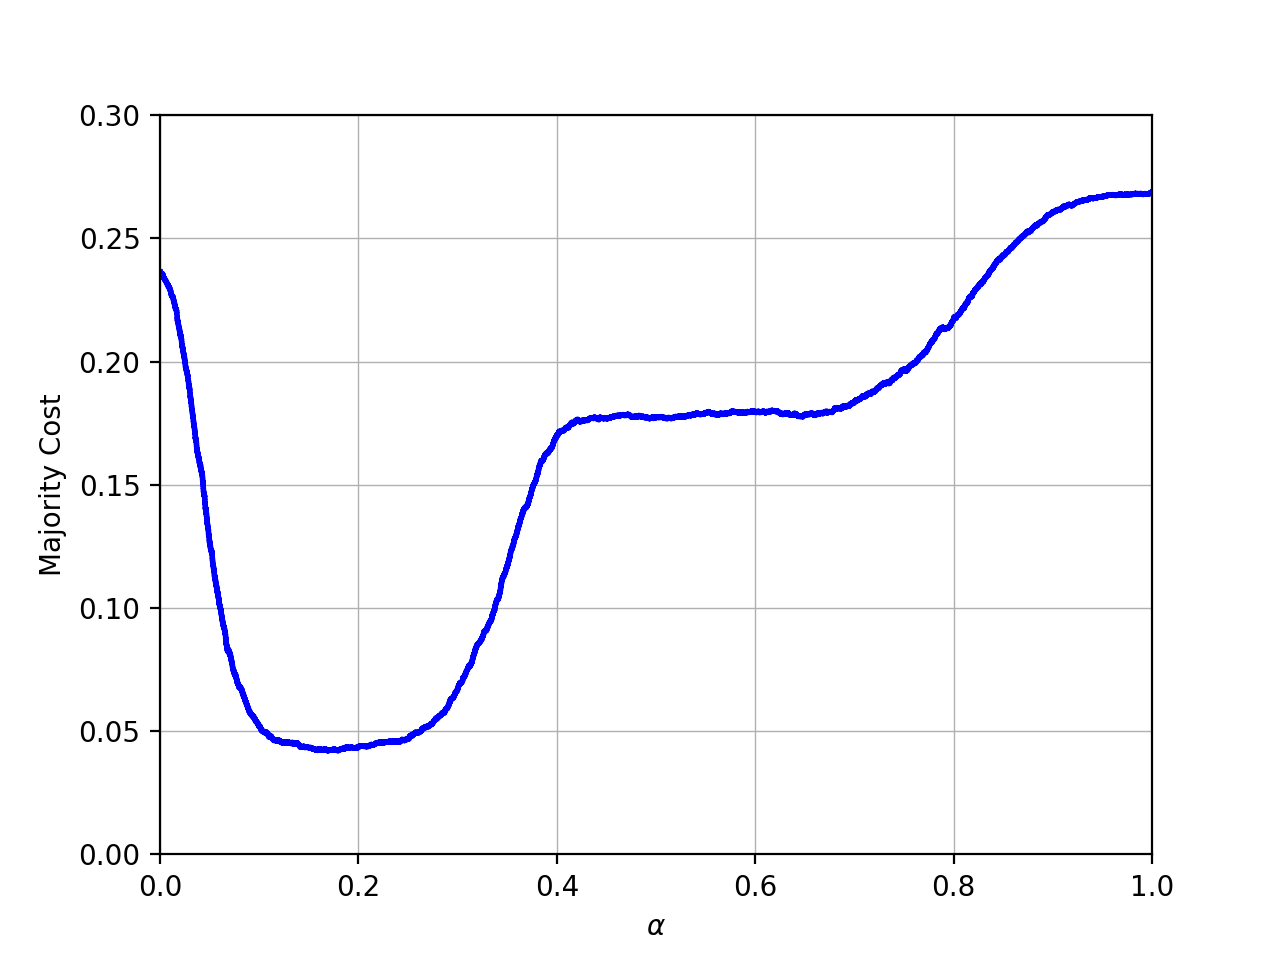
\includegraphics[width=\linewidth]{plots/ringsanddiskssc}}
\end{minipage}\qquad
\begin{minipage}{.45\textwidth}
  \centering
  \subcaptionbox{In comparison, interpolating between average and complete linkage does not lead to improvements. The error stays mostly constant around $26\%$.}
  {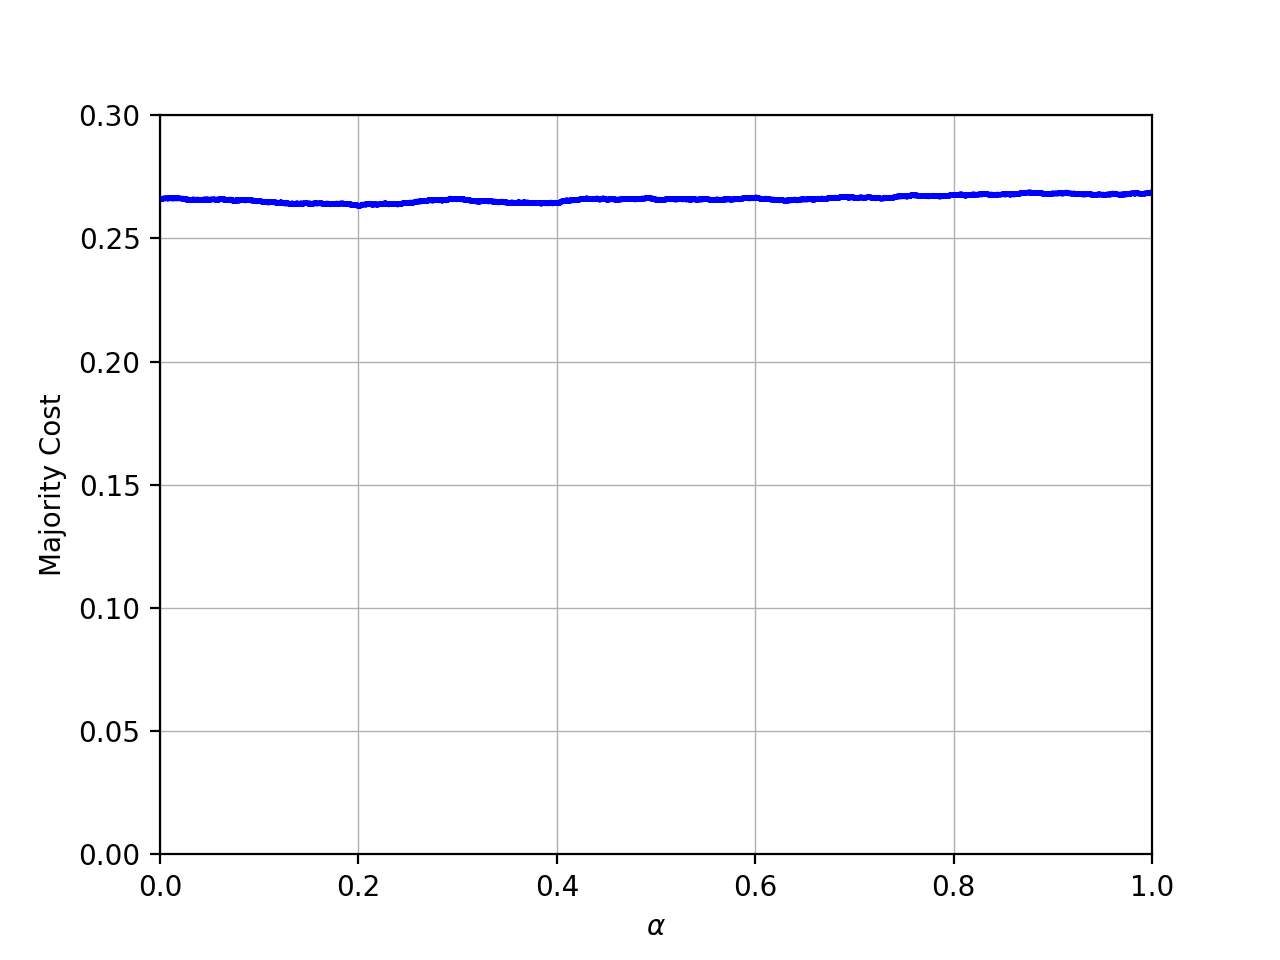
\includegraphics[width=\linewidth]{plots/ringsanddisksac}}
\end{minipage}
\begin{minipage}{.45\textwidth}
  \centering
  \subcaptionbox{Single linkage does well for clustering the rings, however it cannot recognize the clusters in the two disks.}
  {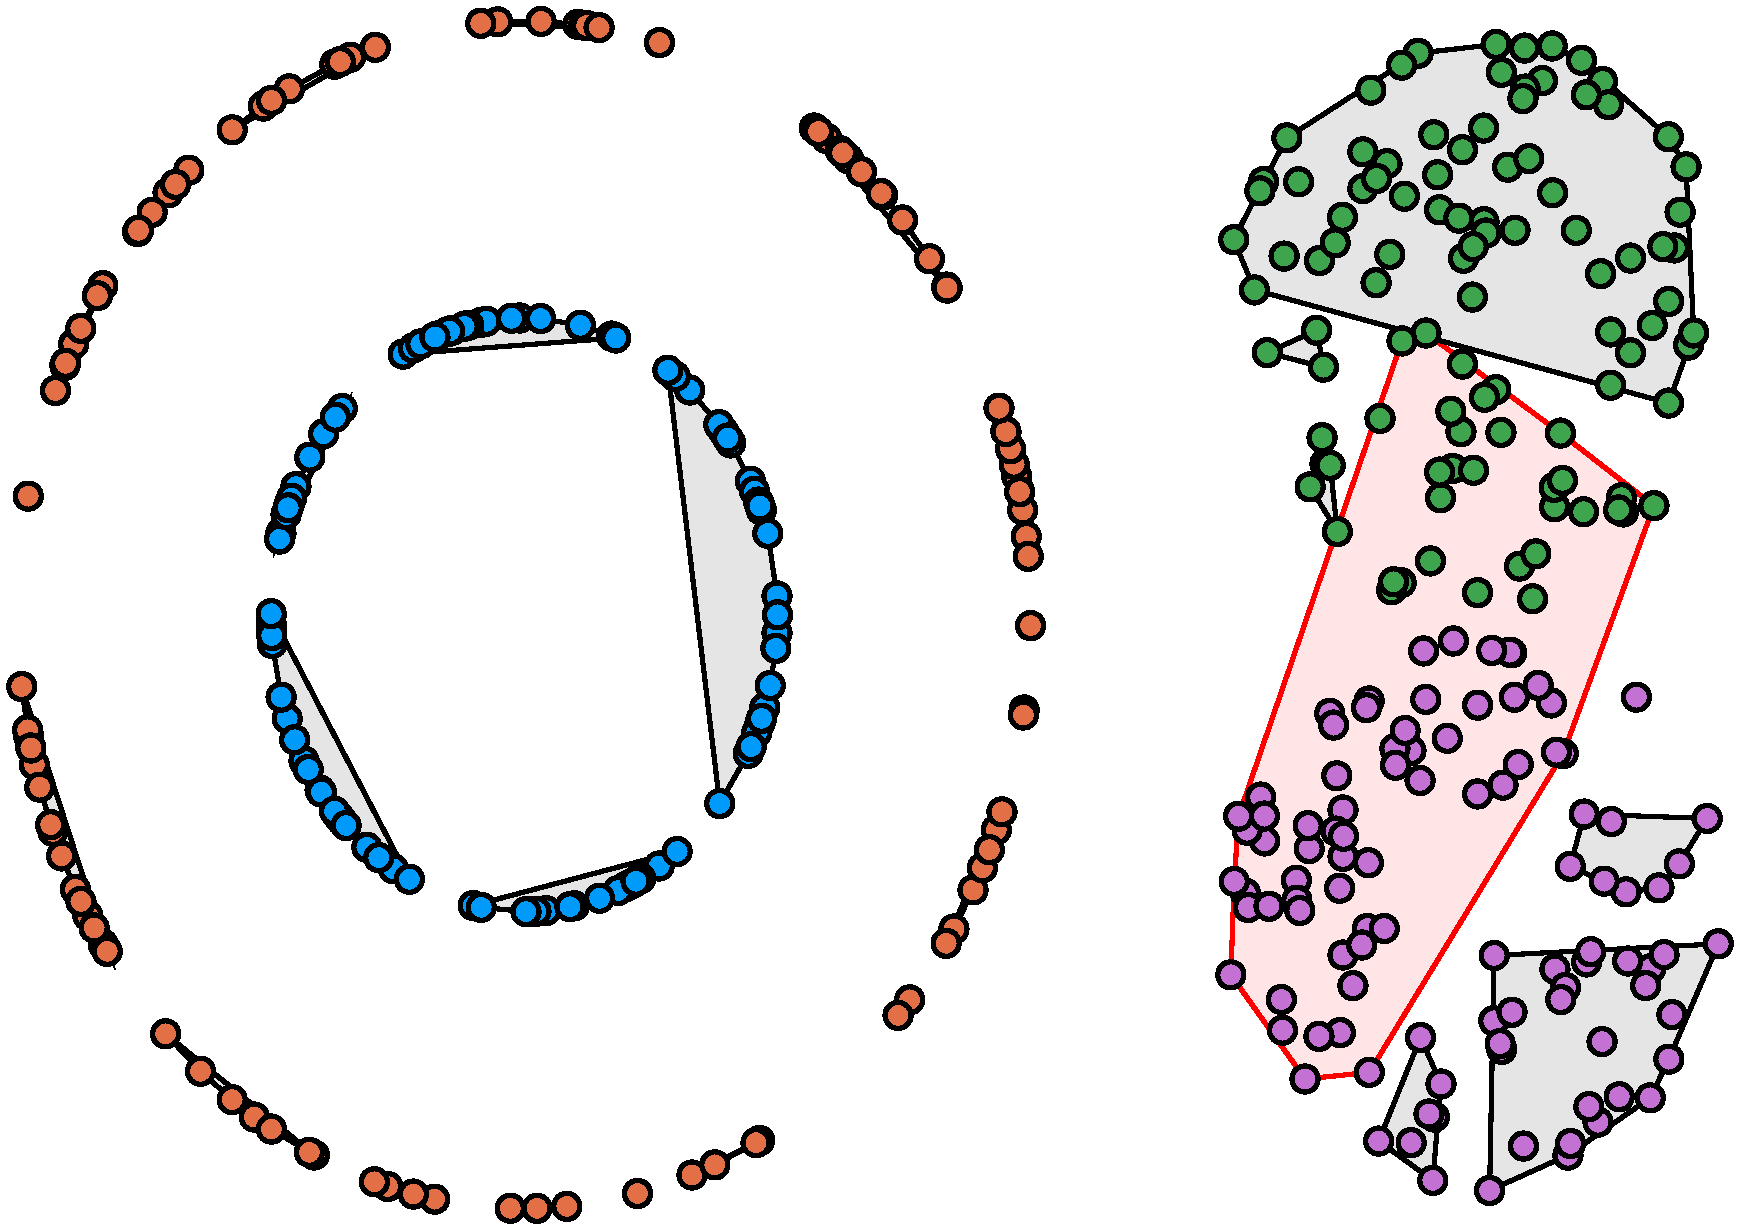
\includegraphics[width=\linewidth]{plots/single_linkage_370}}
\end{minipage}\qquad
\begin{minipage}{.45\textwidth}
  \centering
  \subcaptionbox{Complete linkage does well recognizing the disks, but it fails to correctly identify the rings.}
  {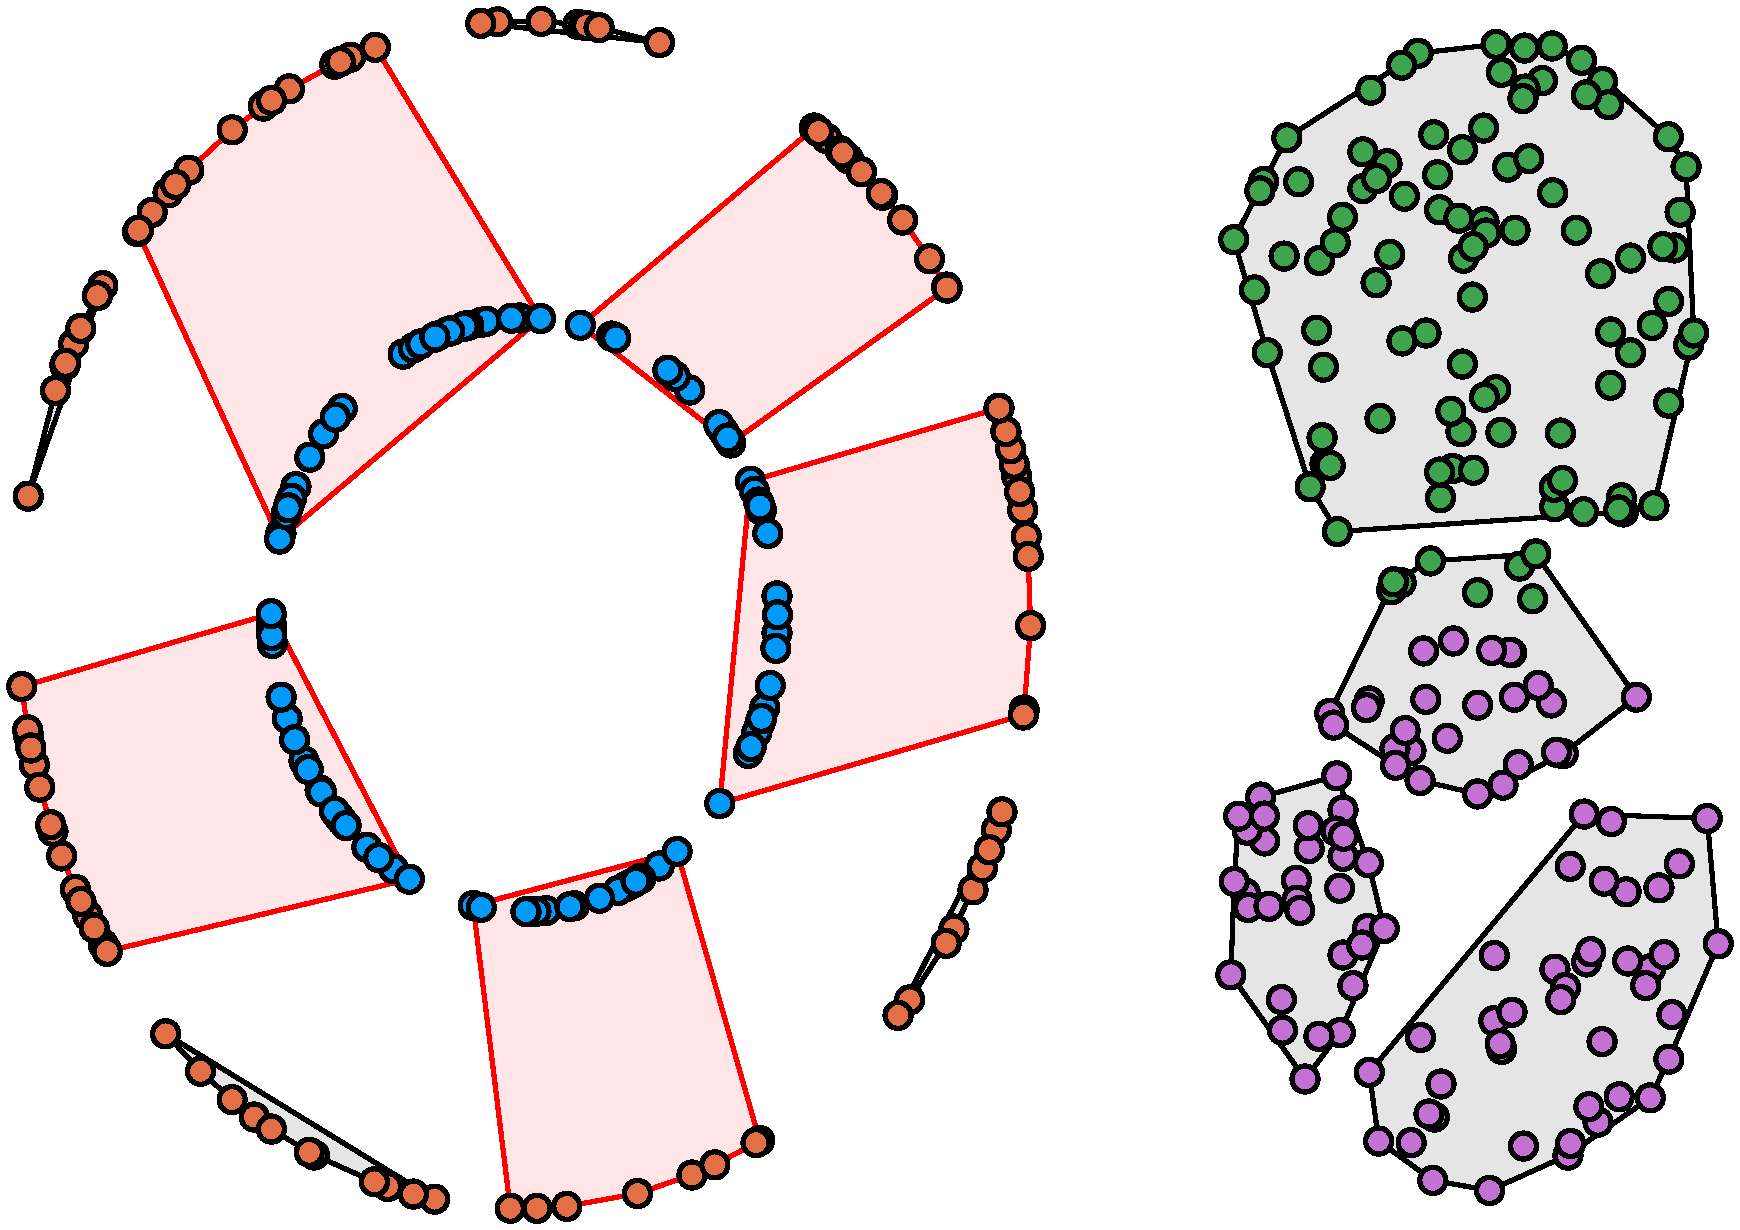
\includegraphics[width=\linewidth]{plots/complete_linkage_389}}
\end{minipage}
\caption{%
  %
  Clustering the synthetic data leads to great improvements when interpolating between single and complete linkage. We observe that single linkage is able to identify the rings very well while complete linkage recognizes the disks. A weighted combination of both is able to process the overall data very well, while average linkage and complete linkage perform almost identically.
  }
  %
\label{fig:syntheticexperiments}
\end{figure}

\subsection{NELL}

In order to find new subclusters for the NELL data, we cluster each of the 32 main categories separately. This results in 32 different clustering tasks, where we compare the results of each clustering task with the target labels using the Majority distance function. We receive a cost function $cost(\alpha)$, that shows us for which value of $\alpha$ the resulting clusterings are good, for each category. By averaging all cost functions, we know for which parameters $\alpha$-linkage performs well in general. Beside having a value of $\alpha$ that can be used for other clustering tasks, the experiments also give different representation levels of clusters. First, we start evaluating all tasks with a maximum of 250 points per task. Figure \ref{fig:nellresults} shows the result for all three different interpolation strategies.

\begin{figure}[h]
\centering
  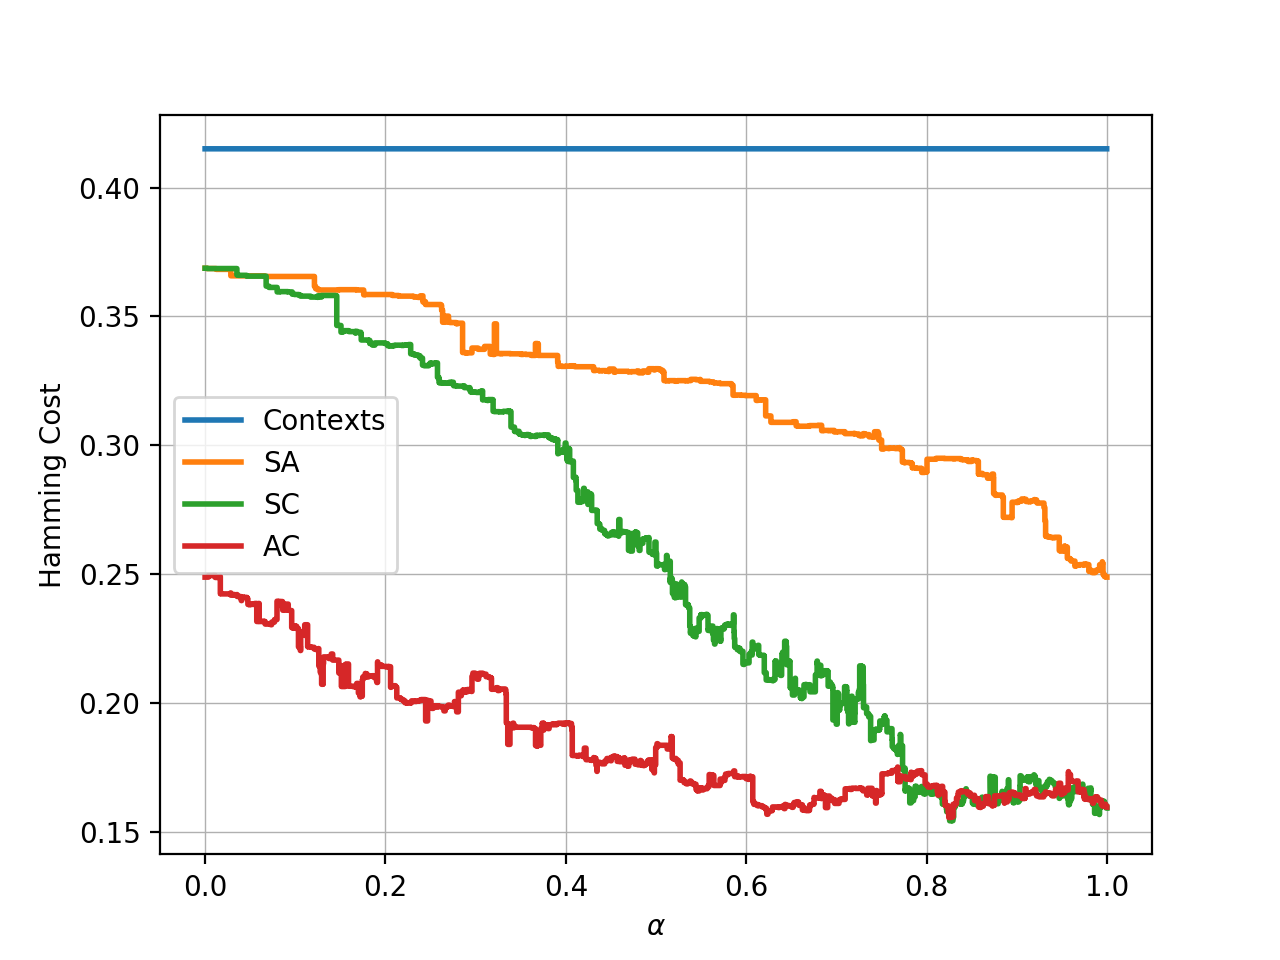
\includegraphics[width=.5\linewidth]{plots/nell_250}
\caption{$\alpha$-linkage using 250 points for each clustering instance gives minor improvements for the NELL data when clustering between single and complete and average and complete linkage. As complete linkage performs best of our input strategies, interpolating between single and average linkage does not lead to improvements.}
\label{fig:nellresults}
\end{figure}

We see minor improvements when clustering between single and complete and average and complete linkage. On the other hand, interpolating between single and average linkage did not lead to any improvement. In order to evaluate the results further, we have a closer look at the curves and see that the overall improvement we get is $0.53\%$, a reduction from $15.97\%$ (complete linkage) to $15.44\%$ ($\dsc(0.826)$) as shown in table \ref{table:nellresults}. An interesting observation is that while single linkage performs very poorly overall, interpolating between single and complete linkage gives a better improvement than interpolating between average and complete linkage. To evaluate these experiments we are using the Majority distance, as for such a large number of target clusters calculating the Hamming distance is not efficient. 

\begin{table}[h]
    \centering
    \begin{tabular}{|l | l|}
    \hline
    Strategy & Majority Cost\\ \hline
    Single Linkage & 0.36871\\
    Average Linkage & 0.248913\\
    Complete Linkage & 0.159725\\
    $\dsc(0.826)$ & 0.154422\\
    $\dac(0.826)$ & 0.155697\\\hline
    \end{tabular}
    \caption{Our proposed algorithm reduces the NELL cost by $\Delta cost = 0.53\%$ when using a maximum of 250 points for each class.}
    \label{table:nellresults}
\end{table}

As the algorithm has become a lot more efficient during this work, we scale up the algorithms to use 1,000 instead of 250 points per class. The results for all entities are shown in appendix \ref{app:nell}. Figure \ref{fig:nellresults1000} shows that in general the error is slightly higher, because our experiments contain more different classes. Overall, we again see slight improvements that are shown in table \ref{table:nell1000}. Compared to the previous experiments, the improvements were slightly larger ($1.21\%$ leading to an error of $16.67\%$), however the overall curves look very similar. In this setting, we also evaluate the parameter advising for the first 10 parameters $\alpha^*$ (see figure \ref{fig:nell1000top10}).

\begin{figure}[h]
\centering
  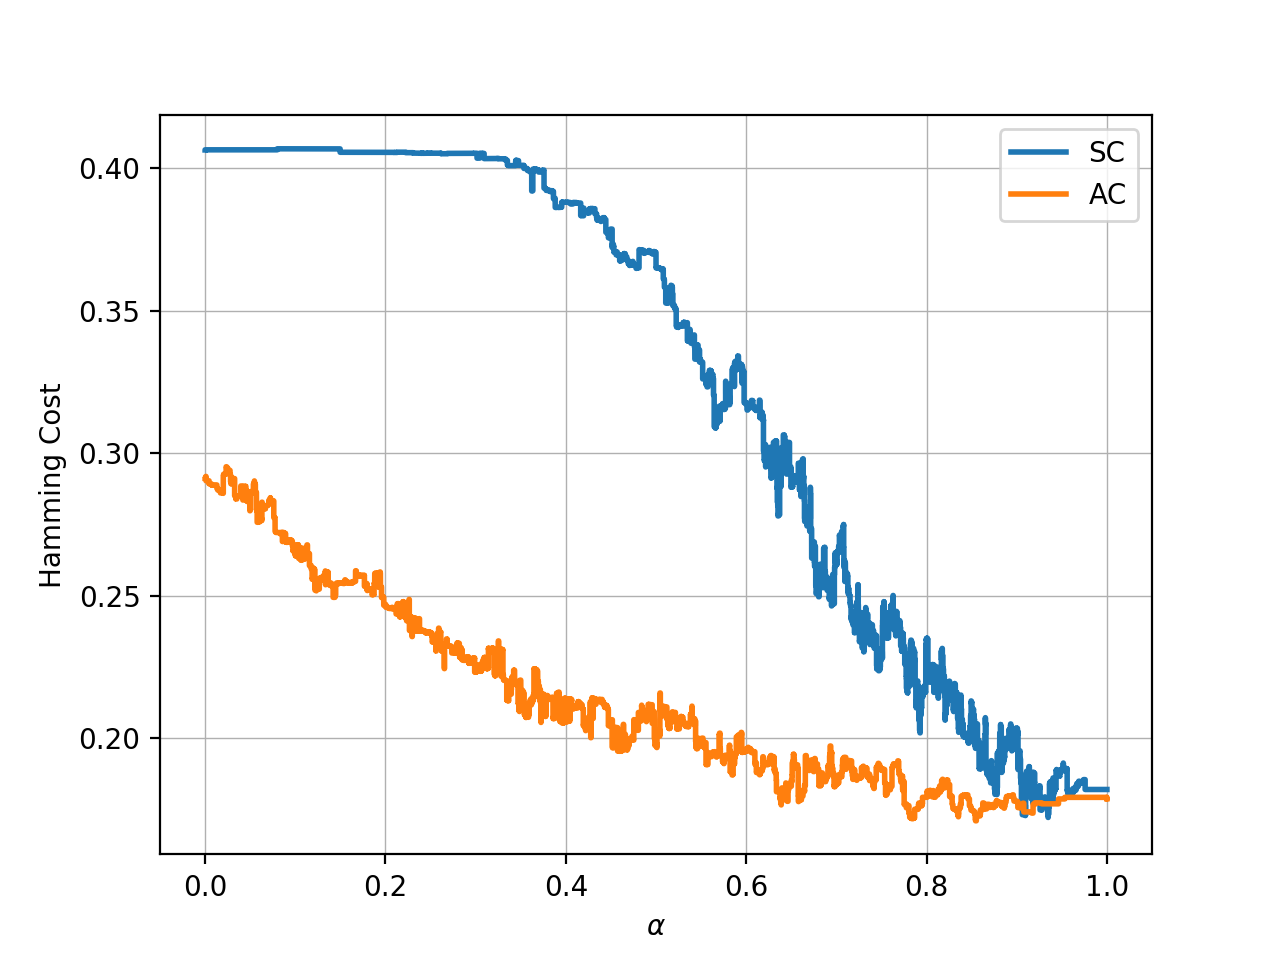
\includegraphics[width=.5\linewidth]{plots/nell_1000}
\caption{$\alpha$-linkage using 1000 points for each clustering instance gives minor improvements for the NELL data when clustering between single and complete and average and complete linkage.}
\label{fig:nellresults1000}
\end{figure}

\begin{table}[h]
    \centering
    \begin{tabular}{|l | l|}
    \hline
    Strategy & Majority Cost\\ \hline
    Single Linkage & 0.36871\\
    Average Linkage & 0.291202\\
    Complete Linkage & 0.17882\\
    $\dsc(0.918)$ & 0.166742\\
    $\dac(0.855)$ & 0.171083\\\hline
    \end{tabular}
    \caption{Our proposed algorithm reduces the NELL cost by $\Delta cost = 1.21\%$ when using a maximum of 1000 points for each class.}
    \label{table:nell1000}
\end{table}

\begin{figure}[h]
\centering
\begin{minipage}{.45\textwidth}
  \centering
  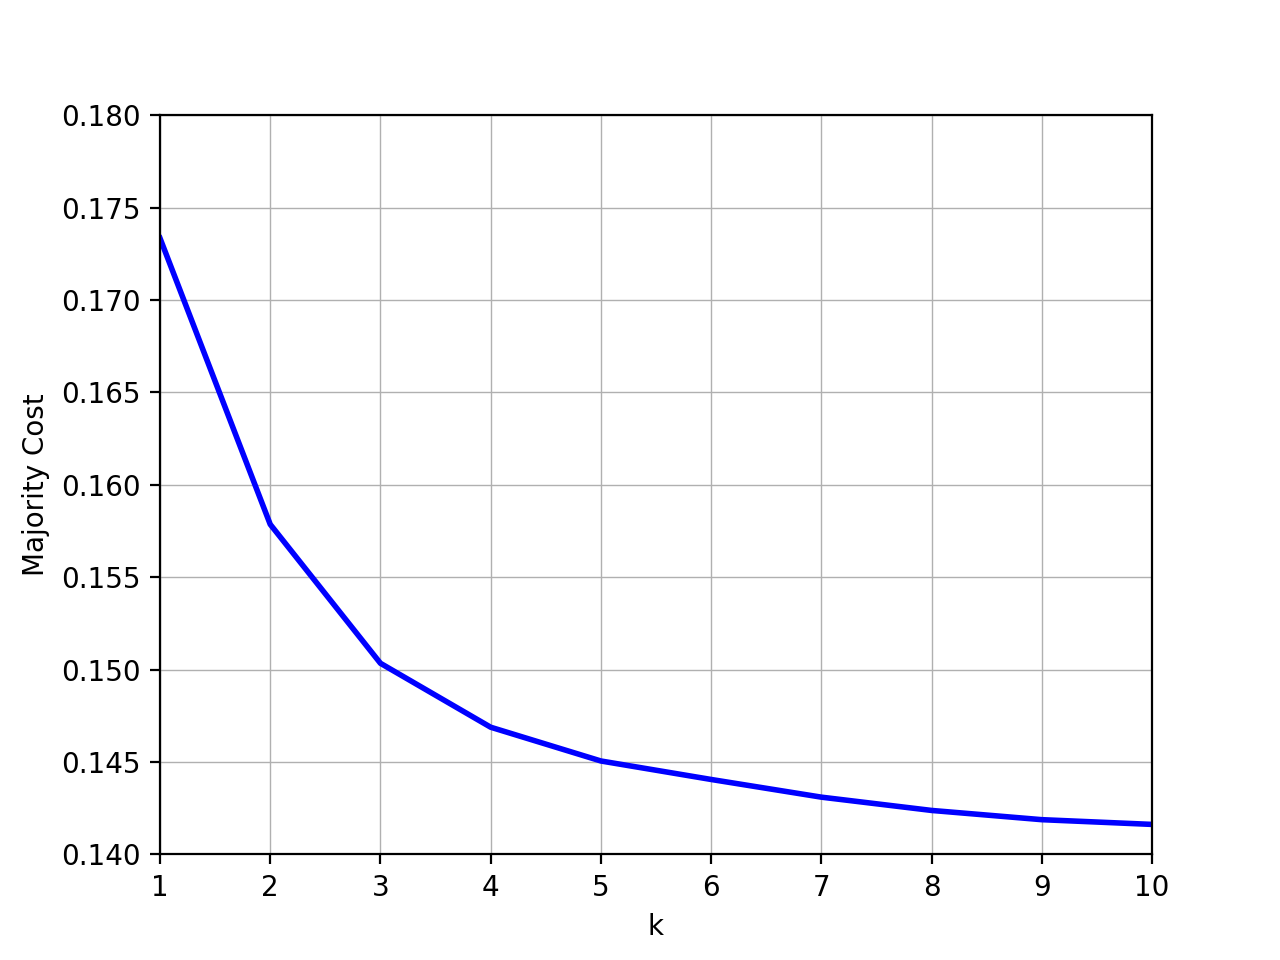
\includegraphics[width=\linewidth]{plots/nell_sc_1000_top10}
\end{minipage}
\begin{minipage}{.45\textwidth}
  \centering
  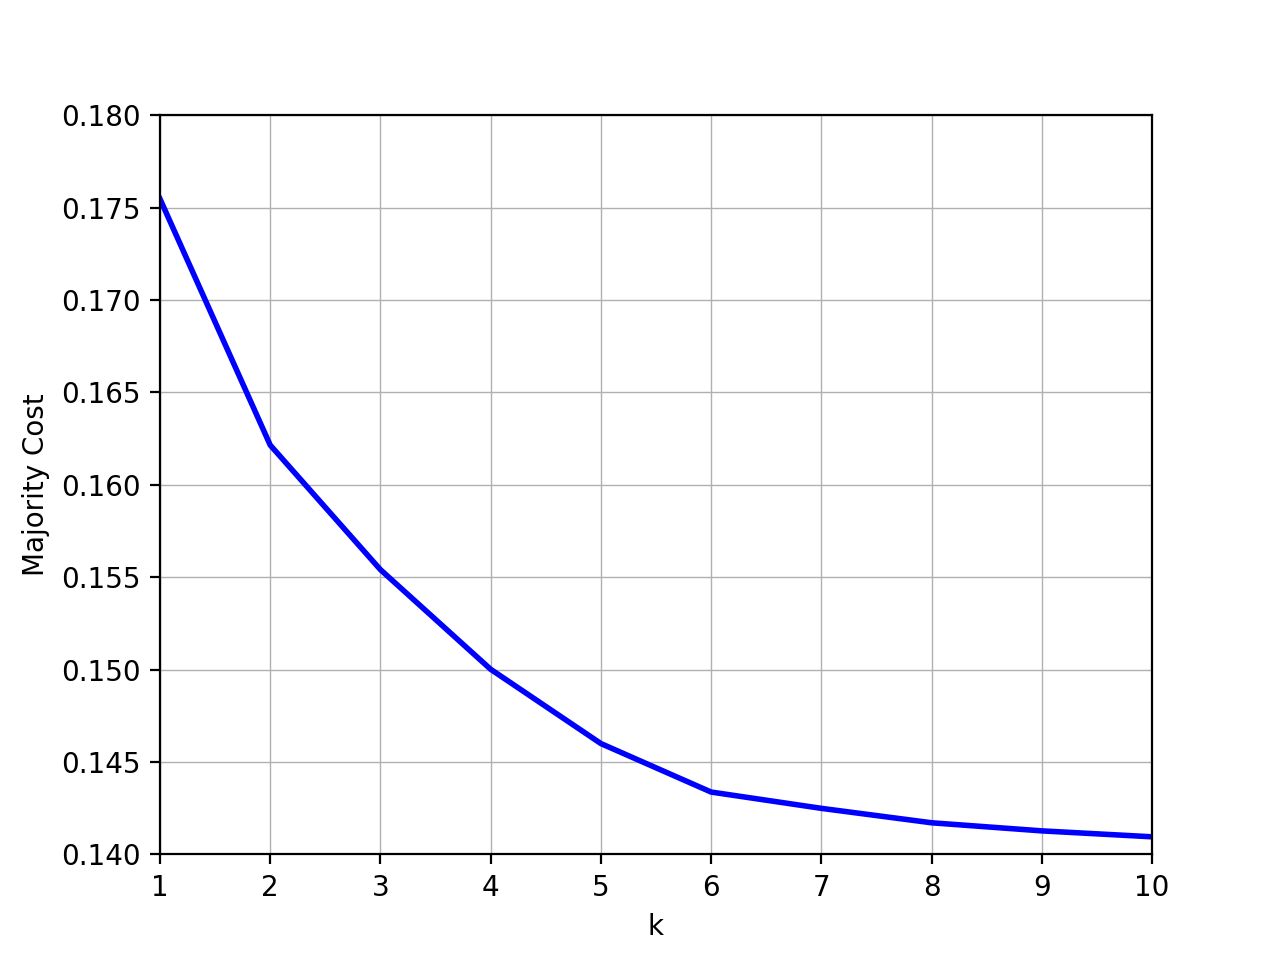
\includegraphics[width=\linewidth]{plots/nell_ac_1000_top10}
\end{minipage}
\caption{Parameter advising improves the clustering in both settings by at least $2\%$ for $k = 3$ parameters $\alpha^*$ for the NELL data.} 
\label{fig:nell1000top10}
\end{figure}

Also, we evaluate the corresponding clusters. As $\alpha$-linkage uses agglomerative hierarchical clustering, we can extract clusters at different levels. Tables \ref{tbl:rooms}, \ref{tbl:clothing} and \ref{tbl:kitchenitems} show some examples for discovered subcategories.

\begin{table}[H]
  \makebox[\textwidth][c]{
  \small
  \begin{tabular}{cccc}
    \hline\hline
    \textbf{Luxury Room} & \textbf{Bathroom} & \textbf{Guest Room} & \textbf{Suite} \\ \hline
    spacious living room & large ensuite bathroom & elegant rooms & luxurious suites\\
    comfortable living room & spacious marble bathroom & three guest rooms & one bedroom suites\\
    guest room & one bathroom & large guest rooms & spacious suites\\
    lounge room & full bathroom & deluxe guest rooms & deluxe suites\\
    living room & upstairs bathroom & guests rooms & guest suites\\
    superior room & large bathroom & spacious air conditioned rooms & bedroom suites\\
    sleeping room & ensuite bathroom & furnished guest rooms & whirlpool suites\\
    main bedroom & elegant bathroom & comfortable guest rooms & three suites\\
    \hline
  \end{tabular}
  }
  \caption{Proposed subcategories for ``Office Building Room''.}
  \label{tbl:rooms}
\end{table}

\begin{table}[H]
  \makebox[\textwidth][c]{
  \small
  \begin{tabular}{ccccc}
    \hline\hline
    \textbf{Shoes} & \textbf{Uniform/Costume} & \textbf{Pants} & \textbf{Casual} & \textbf{Specialized} \\ \hline
    shoes & costume & kneepants & stocking cap & long stockings\\
    high heel shoes & work uniforms & baggy pants & workout clothes & wide brimmed hat\\
    sensible shoes & outfits & loose fitting pants & casual clothes & casual wear\\
    old shoes & period costume & slacks & baseball caps & black stockings\\
    pointe shoes & folk costumes & black shorts & skull caps & wear socks\\
    dark shoes & halter top & special clothing & ball caps & high heels\\
    spira shoes & period costumes & white shorts & evening clothes & surf wear\\
    mens shoes & costumes & underpants & ball cap & wear gloves\\
    \hline
  \end{tabular}
  }
  \caption{Proposed subcategories for ``Clothing''.}
  \label{tbl:clothing}
\end{table}

\begin{table}[H]
  \makebox[\textwidth][c]{
  \small
  \begin{tabular}{cccc}
    \hline\hline
    \textbf{Stove/Oven} & \textbf{Machines} & \textbf{Bowls} & \textbf{Baking Sheets} \\ \hline
    full size stove & cookie cutters & large mixing bowl & oiled baking sheet\\
    full size cooker & automatic washing machine & large serving bowl & rimmed baking sheet\\
    red hot stove & washing machine & small bowl & large baking sheet\\
    plastic jug & bread machine & single bowl & small baking sheet\\
    toaster & cookie cutter & separate bowl & prepared baking sheet\\
    greased baking dish & coffee machine & shallow bowl & ungreased baking sheet\\
    wood burning pizza oven & cooking spray & separate mixing bowl & hot plate\\
    ceramic top stove & coffee grinder & large bowl & greased baking sheet\\
    \hline
  \end{tabular}
  }
  \caption{Proposed subcategories for ``Kitchen Item''.}
  \label{tbl:kitchenitems}
\end{table}

\paragraph{Bag-of-Contexts.} In addition to using the original features, we also use the bag-of-contexts representations to evaluate these experiments. The features are represented in a sparse very high-dimensional dataset. The feature representation leads to a constant error of $\approx 41\%$ as shown in figure \ref{fig:nellresults}, i.e.\ this feature representation did not lead to improvements over the existing feature representation that was created by domain experts. Also, the error stays constant for all three discussed linkage strategies as well as the interpolation between them. This means that the feature representation does not lead to good clusterings and $\alpha$-linkage can not overcome the problem in this case.

\subsection{MNIST}

\paragraph{Pixel Representation.} For the MNIST images, we evaluate both described experimental settings with combinations of five out of the ten target classes. To cluster the data, we set up $10 \choose 5$ $= 252$ different experiments by selecting all combinations of five out of the ten labels. In order to do so in efficient time, we subsample the dataset to 200 points for each label, so one experiment will cluster 1000 points. First, we evaluate the results for both average to complete and single to complete linkage for several batches. We show the experiments for the six first batches $b_i, i \in \{0, 1, 2, 3, 4, 5\}$ for interpolating between single and complete linkage.

\begin{figure}[h]
\centering
\begin{minipage}{.45\textwidth}
  \centering
  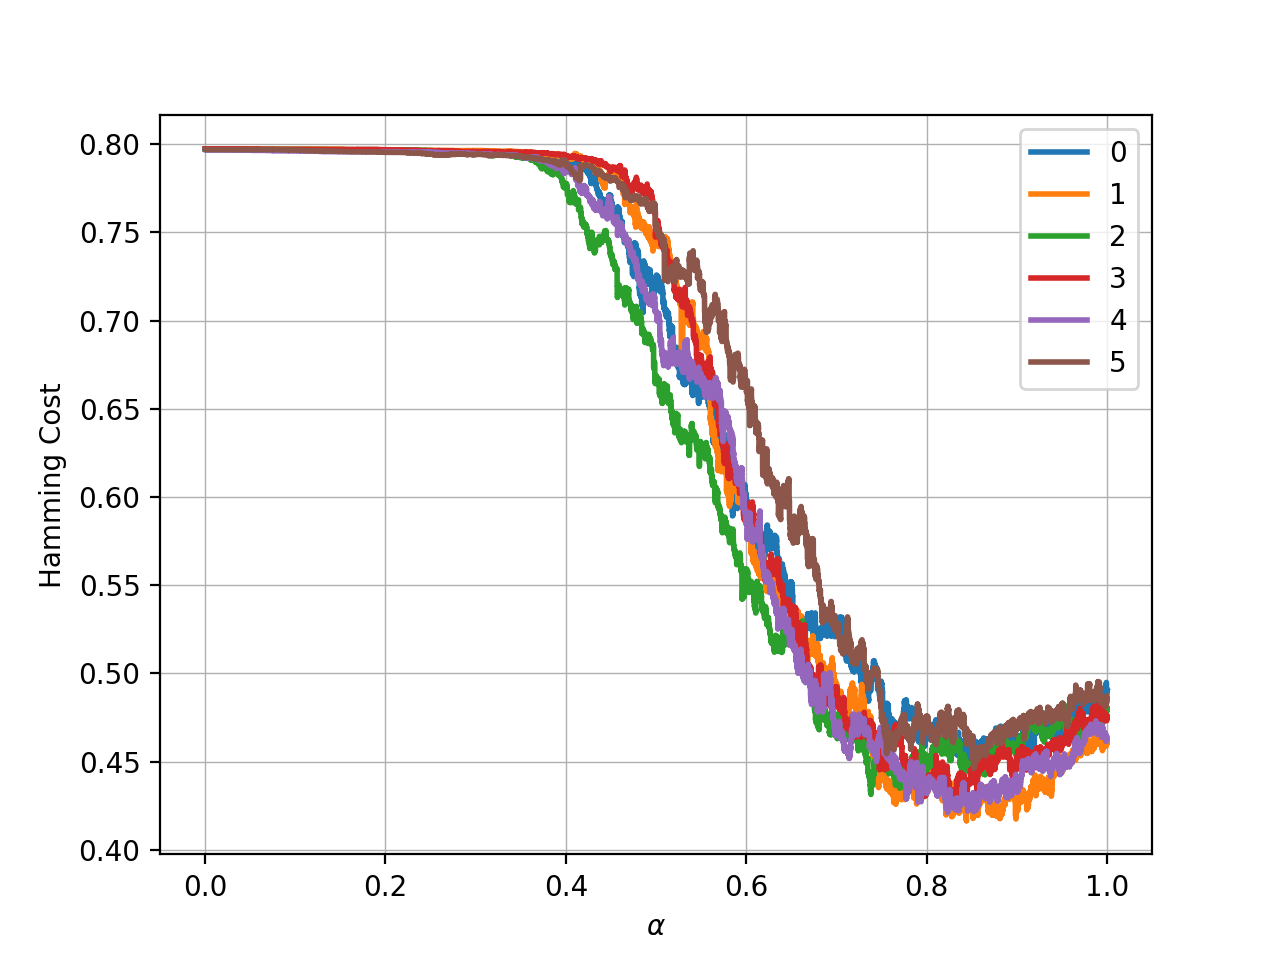
\includegraphics[width=\linewidth]{plots/mnist_sc_all_batches}
\end{minipage}
\begin{minipage}{.45\textwidth}
  \centering
  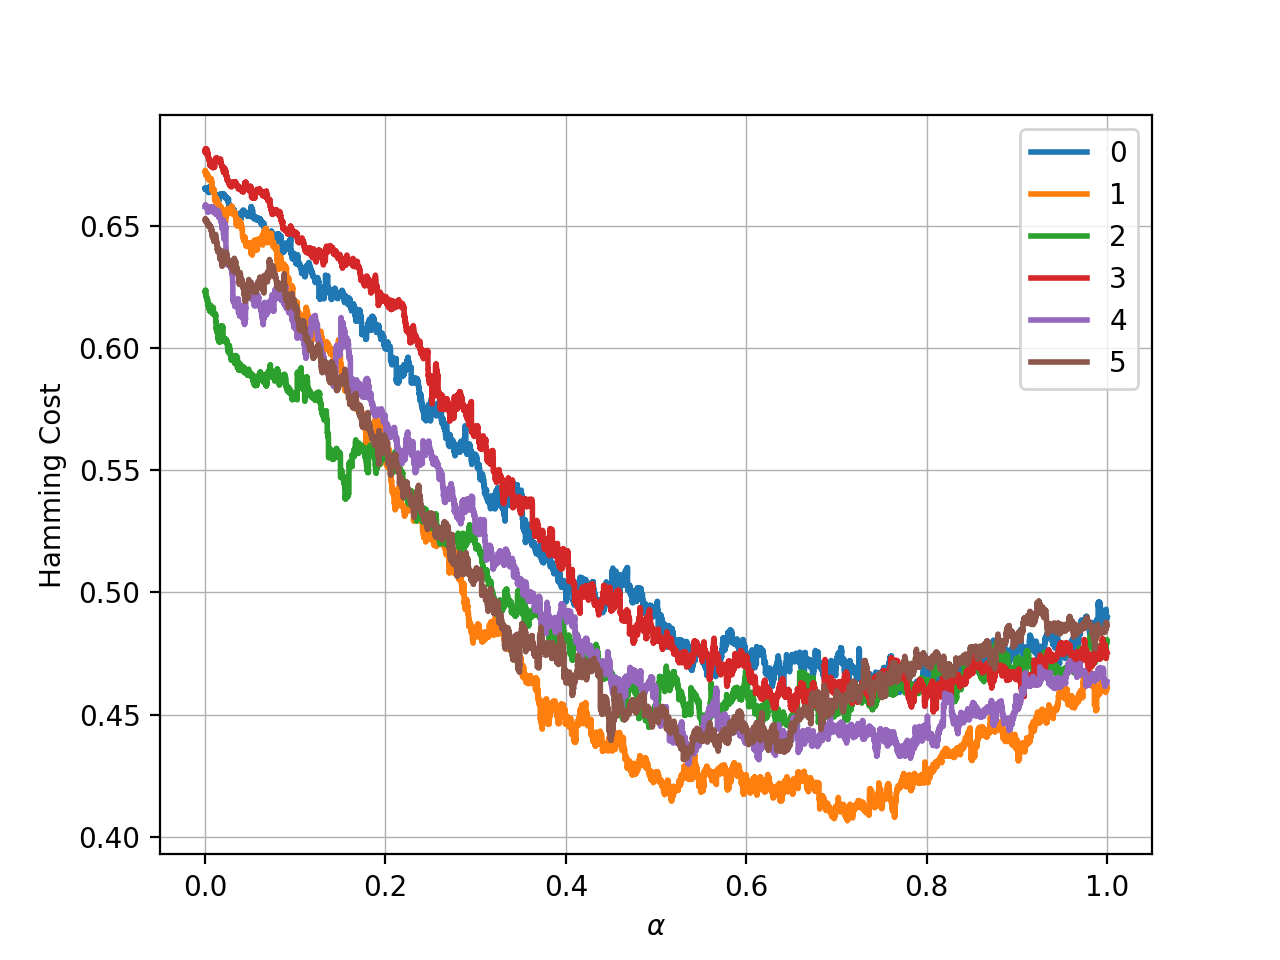
\includegraphics[width=\linewidth]{plots/mnist_ac_all_batches}
\end{minipage}
\caption{Over the first six batches of the MNIST data, interpolating between single and complete linkage shows a similar behavior (left) while interpolating between average and complete linkage leads to bigger differences (right).}
\label{fig:mnistbatches}
\end{figure}

As shown in figure \ref{fig:mnistbatches} (left), the clustering over the first six batches leads to very similar curves with slightly different errors. Table \ref{table:mnistscbatches} evaluates the results in more detail.

\begin{table}[H]
    \centering
    \begin{tabular}{|l | l l l l l l |}
    \hline
    Strategy & Batch 0 & Batch 1 & Batch 2 & Batch 3 & Batch 4 & Batch 5\\ \hline
    Single Linkage & 0.796901 & 0.797345 & 0.797171 & 0.797405 & 0.796766 & 0.797024\\
    Complete Linkage & 0.490468 & 0.461063 & 0.479825 & 0.475329 & 0.463321 & 0.487111\\
    $\alpha_{opt}$ & 0.87228 & 0.84419 & 0.778498 & 0.83199 & 0.82338 & 0.852251\\
    $cost_{opt}$ & 0.450012 & 0.416433 & 0.431143 & 0.423786 & 0.421103 & 0.446032\\
    $\Delta cost$ & 4.0456\% & 4.463\% & 4.8682\% & 5.1543\% & 4.2218\% & 4.1079\%\\\hline
    \end{tabular}
    \caption{$\alpha$-linkage reduces the cost of the MNIST dataset by up to $\Delta cost = 5.1543\%$ when interpolating between single and complete linkage.}
    \label{table:mnistscbatches}
\end{table}

Table \ref{table:mnistscbatches} leads to several observations. Clustering points of five classes with a random guess will result in an error of $80\%$. As for all batches single linkage results in an error between $79\%$ and $80\%$, we note that single linkage performs similar as a random guess would. Thus, single linkage is not suitable for the MNIST data. In comparison, complete linkage results in errors below $50\%$ on just using the pixel data. It is not necessarily a great result, but it indicates that grouping high-dimensional pixel features with unsupervised learning can work. Also, we note that the parameter $\alpha_{opt}$ does not vary much and also we notice in figure \ref{fig:mnistbatches} that for $\alpha \in [0.75,1.0)$ we outperform complete linkage in all cases. As the results are very similar for the used batches, we also average over the batches in figure \ref{fig:mnist_overview}. After we evaluate six batches with 252 experiments each, we have a solid base to compare how the different interpolation strategies behave. In figure \ref{fig:splits} we show the overall amount of discontinuities in a histogram for interpolating between single and complete and between average and complete linkage. Also, we show a histogram that indicates how many splits happen in given regions for the value $\alpha$.

\begin{figure}[h]
\centering
\begin{minipage}{.45\textwidth}
  \centering
  \subcaptionbox{Interpolating between average and complete linkage results in 27,000 - 35,000 discontinuities.}
  {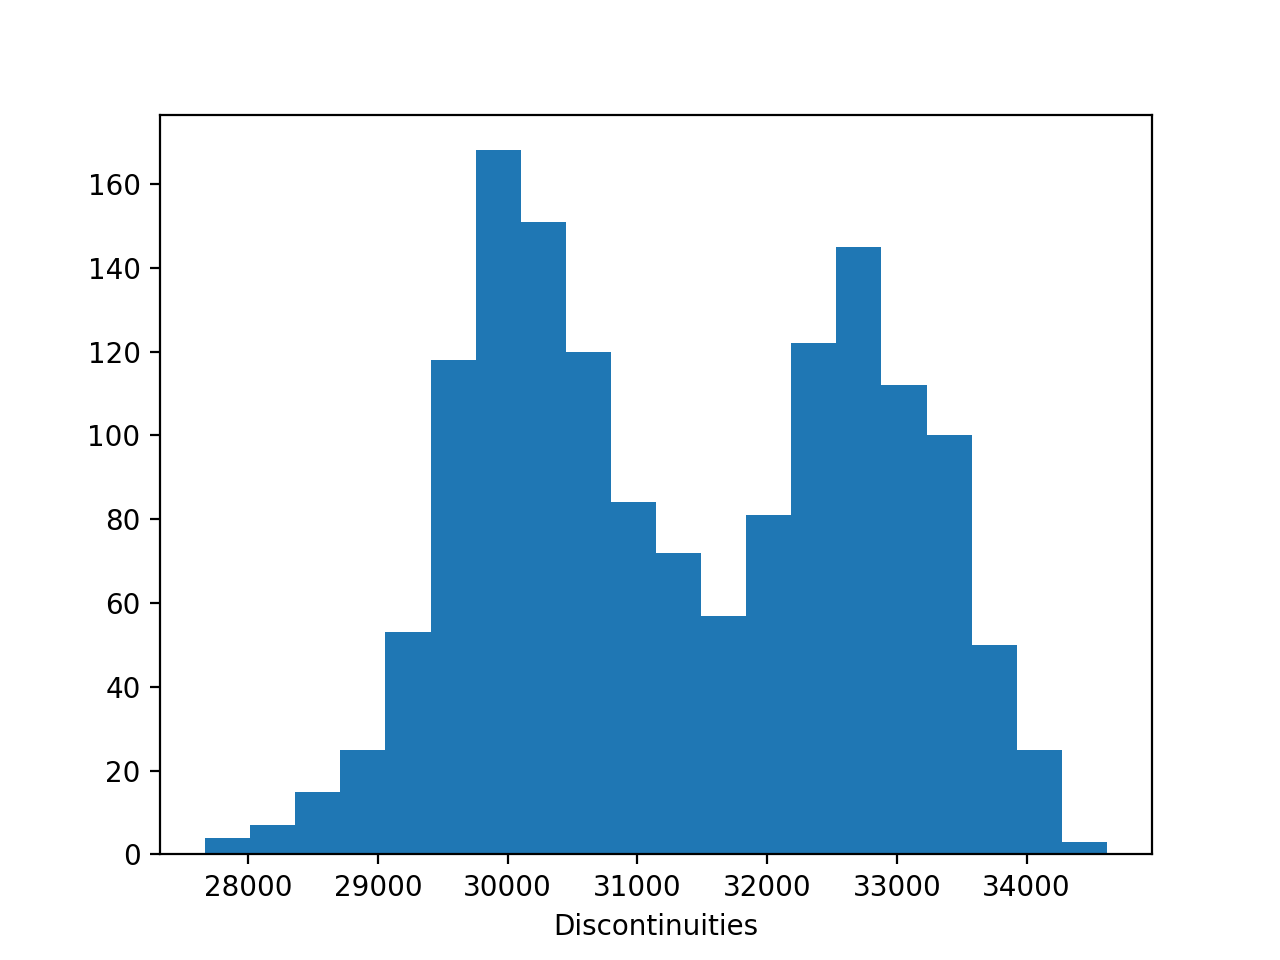
\includegraphics[width=\linewidth]{plots/mnist_ac_splits}}
\end{minipage}\quad
\begin{minipage}{.45\textwidth}
  \centering
  \subcaptionbox{Interpolating between single and complete linkage results in at least 100,000 discontinuities.}
  {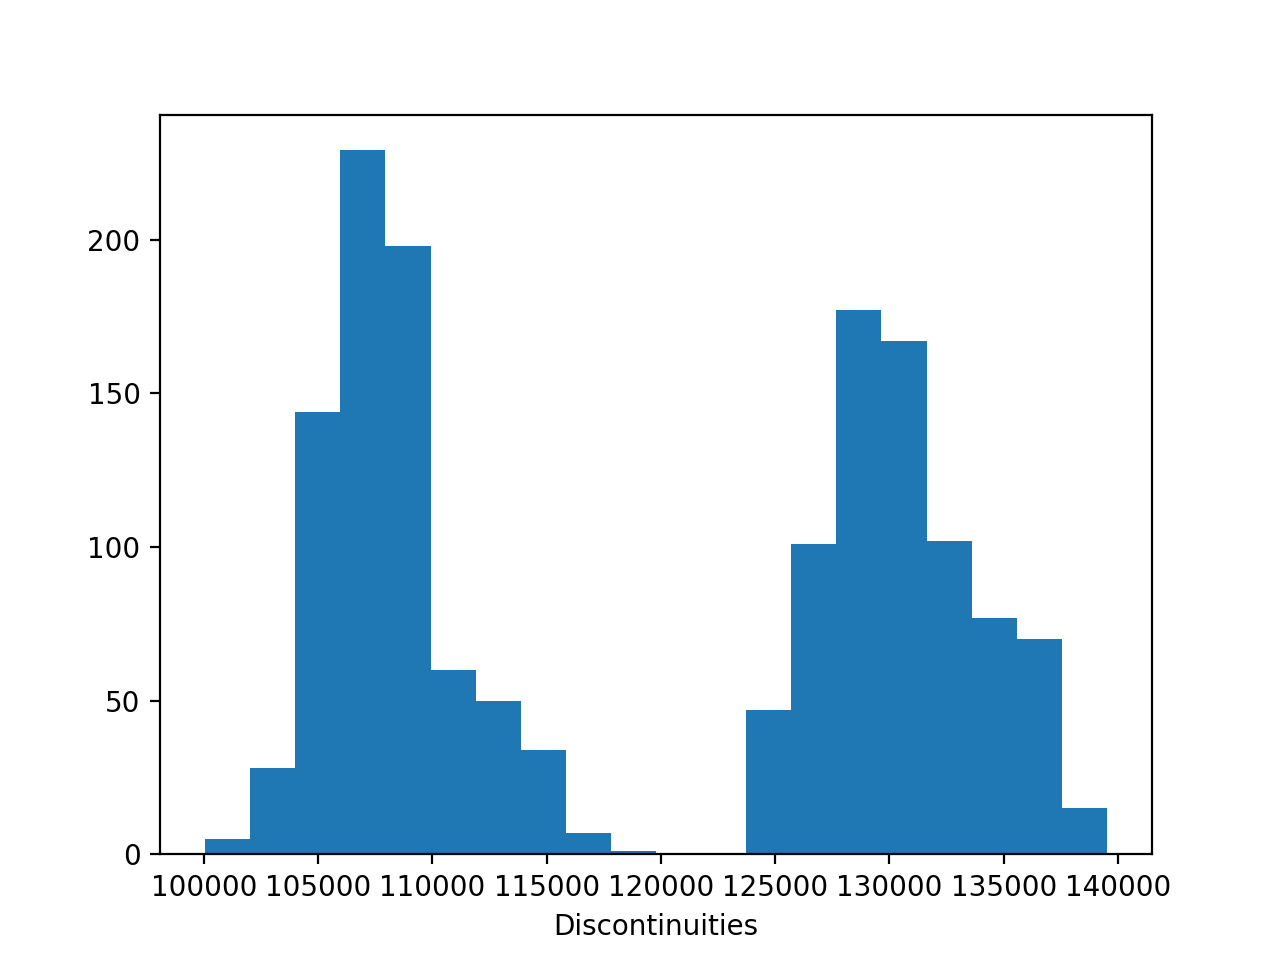
\includegraphics[width=\linewidth]{plots/mnist_sc_splits}}
\end{minipage}
\begin{minipage}{.45\textwidth}
  \centering
  \subcaptionbox{The amount of discontinuities is linearly decreasing when interpolating between average and complete linkage.}
  {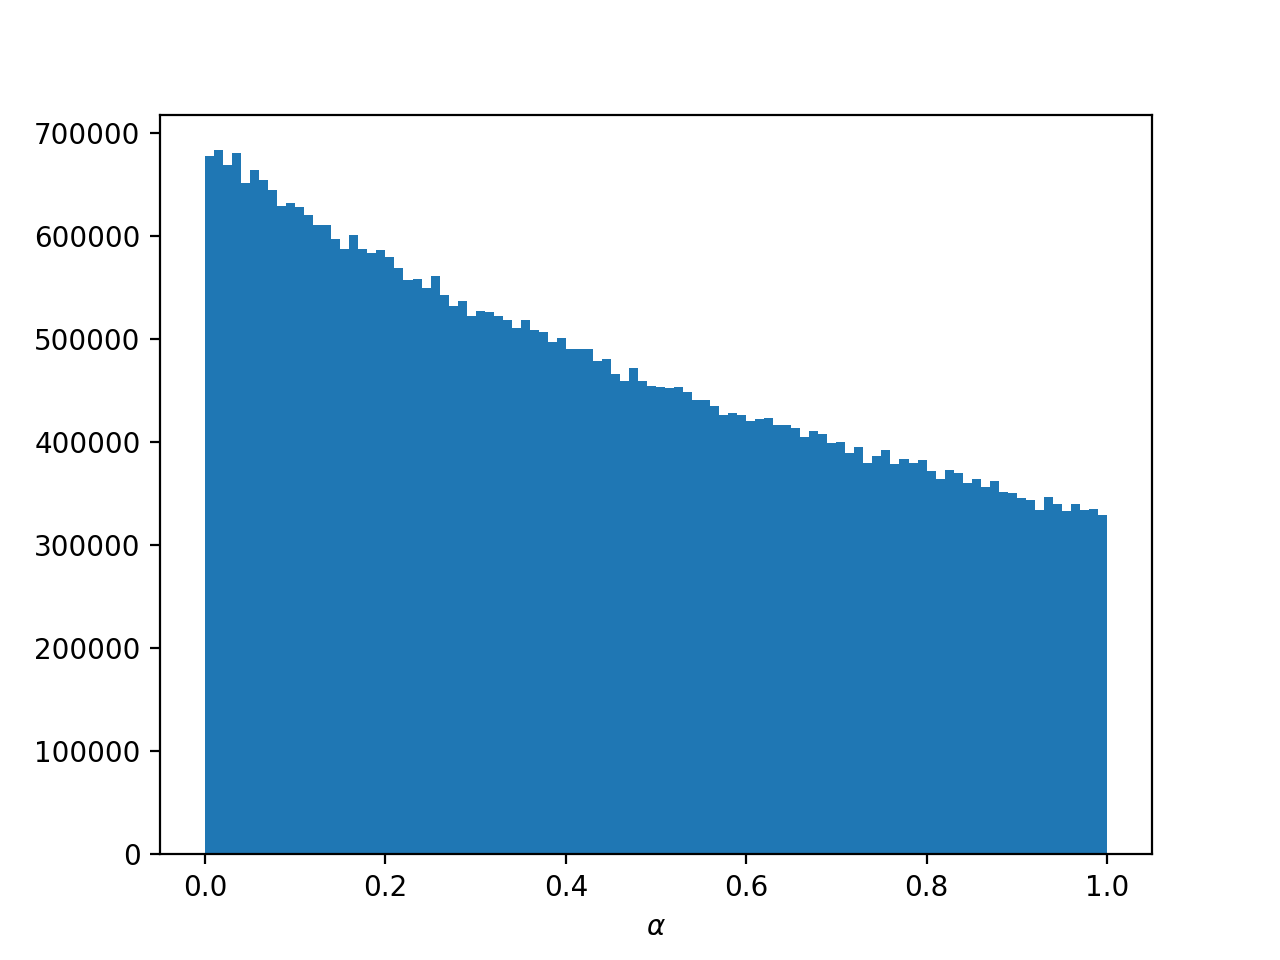
\includegraphics[width=\linewidth]{plots/mnist_ac_split_counts}}
\end{minipage}\quad
\begin{minipage}{.45\textwidth}
  \centering
  \subcaptionbox{The amount of discontinuities is exponentially decreasing when interpolating between single and complete linkage.}
  {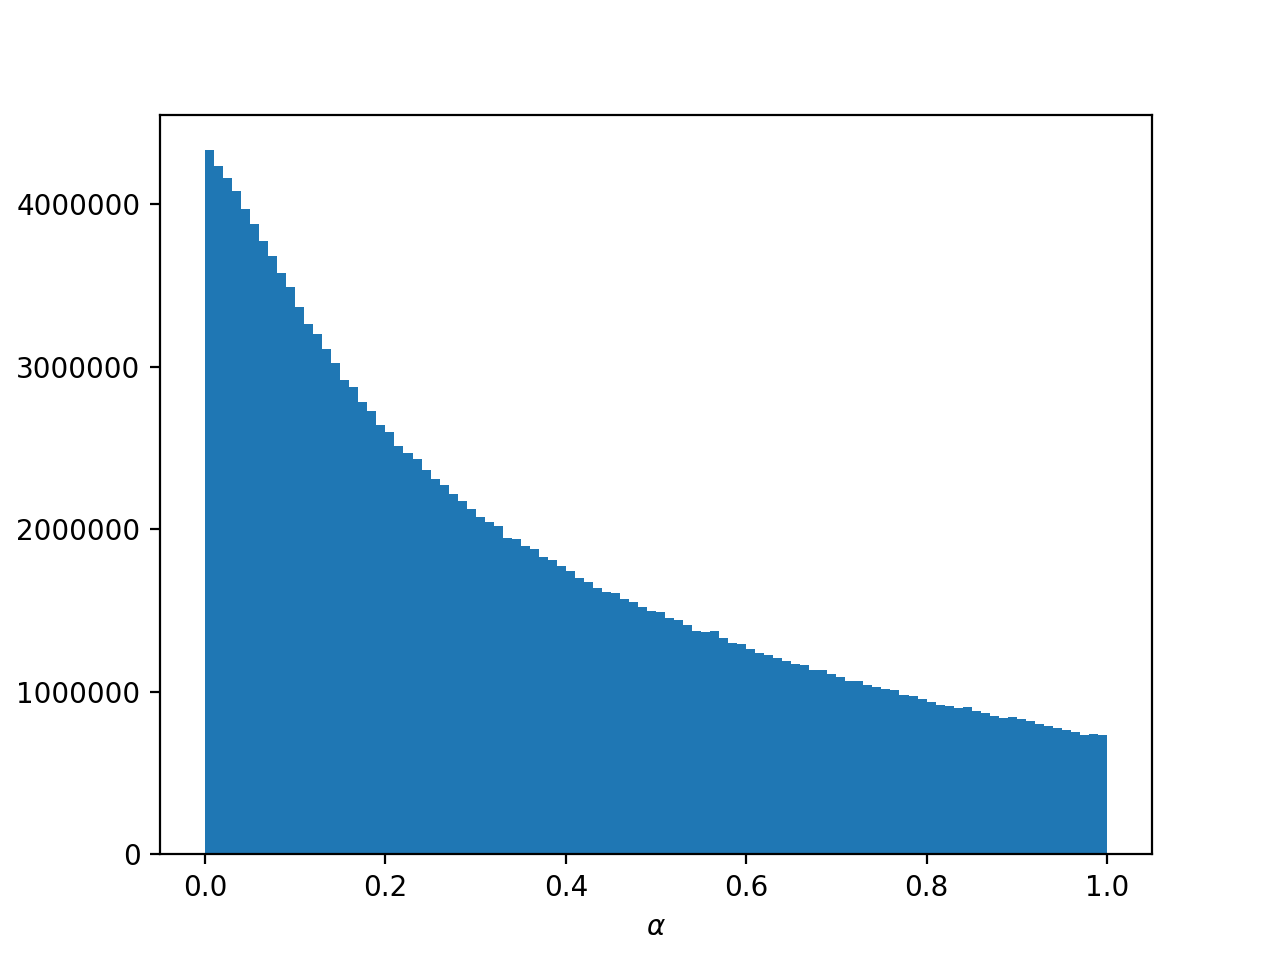
\includegraphics[width=\linewidth]{plots/mnist_sc_split_counts}}
\end{minipage}
\caption{Interpolating between single and complete linkage leads to more than three times as many discontinuities for the MNIST batch experiments as interpolating between average and complete linkage. More discontinuities happen close to single linkage.}
\label{fig:splits}
\end{figure}

In figure \ref{fig:splits} we observe that interpolating between single and complete linkage leads to a larger amount of discontinuities than interpolating between average and complete linkage, when evaluating the MNIST batch experiments it is more than three times as many. We also observe that a large amount of discontinuities occurs close to single linkage, i.e.\ we observe a huge variety of different clustering trees. Precisely, around single linkage ($\alpha \rightarrow 0$) we observe four times as many different clusterings as for complete linkage ($\alpha \rightarrow 1$). An interesting observation is that for $\alpha \approx 0.25$ we have half as many discontinuities as for single linkage and twice as many as complete linkage, i.e.\ we have an approximately exponential decrease during the interpolation.\\

Figure \ref{fig:mnist_overview} and table \ref{table:mnist1000avgsc} show that by applying $\alpha$-linkage interpolating between single and complete linkage, we improve the Hamming cost by $3.7\%$ over the first six data batches, i.e. the first 12,000 points of the dataset. Next, we evaluate the randomized experiments for the same interpolation method, where we average over 512 experiments that are run with random label subsets and randomly selected points for each of the selected labels. Figure \ref{fig:mnistscrandom} shows that in this setting we obtain a very similar curve as in the other setting.

\begin{table}[H]
    \centering
    \begin{tabular}{|l | l |}
    \hline
    Strategy & Hamming Cost\\ \hline
    Single Linkage & 0.797102\\
    Complete Linkage & 0.476186\\
    $\alpha_{opt}$ & 0.857\\
    $cost_{opt}$ & 0.439207\\
    $\Delta cost$ & 3.6979\%\\\hline
    \end{tabular}
    \caption{Over the first 12,000 points of the MNIST dataset interpolating between single and complete linkage improves the Hamming cost by $3.7\%$.}
    \label{table:mnist1000avgsc}
\end{table}

\begin{figure}[h]
    \centering
    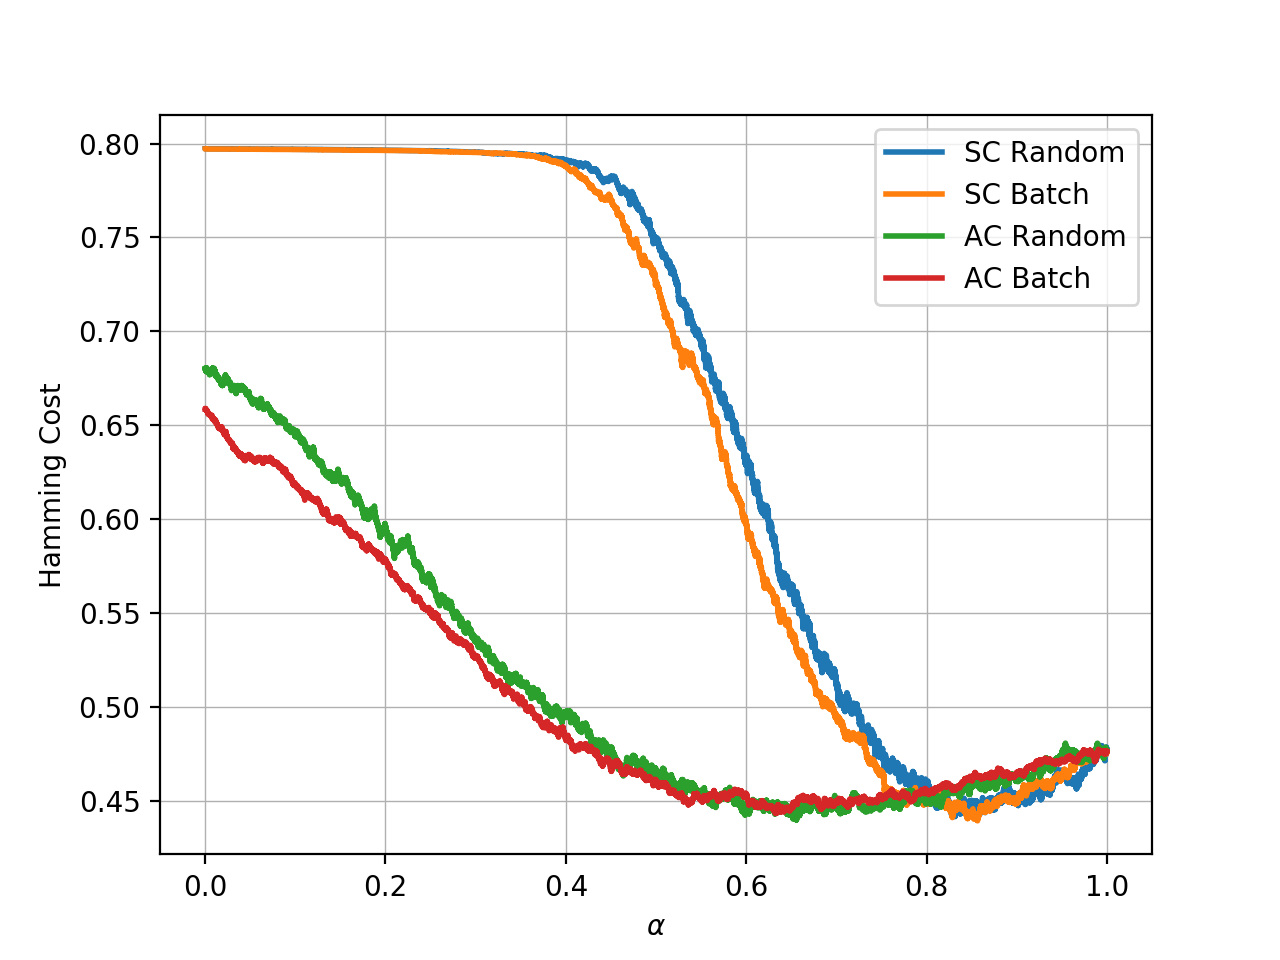
\includegraphics[width=0.5\textwidth]{plots/mnist_1000.png}
    \caption{Comparing the averaged batch and the random settings leads to very similar curves for interpolating between single and complete and between average and complete linkage.}
    \label{fig:mnistscrandom}
\end{figure}

Table \ref{table:mnist1000randomsc} compares the results for both settings when interpolating between single and complete linkage. We obtain very similar results for single and complete linkage. Also, the optimal parameter $\alpha_{opt}$ is the same in both settings leading to similar improvements in the Hamming cost. This means that $\alpha$-linkage is robust over the entire MNIST distribution and with an improvement of more than $3\%$ towards complete linkage it outperforms both used linkage strategies by a major difference. In addition, we also evaluate the greedy parameter advising for the previous experiments. By using $k = 3$ parameters $\alpha^*$ the cost drops more than $5\%$ in addition to less than $38\%$. In comparison to the best linkage strategy, i.e. complete linkage, this is an improvement of $\approx 10\%$.

\begin{table}[H]
    \centering
    \begin{tabular}{|l | l | l |}
    \hline
    Strategy & Hamming Cost (Batch) & Hamming Cost (Random)\\ \hline
    Single Linkage & 0.797102 & 0.797215\\
    Complete Linkage & 0.476186 & 0.476355\\
    $\alpha_{opt}$ & 0.857 & 0.857\\
    $cost_{opt}$ & 0.439207 & 0.440932\\
    $\Delta cost$ & 3.6979\% & 3.5423\%\\\hline
    \end{tabular}
    \caption{Evaluating the randomized setting leads to exactly the same parameter $\alpha_{opt}$ and a similar cost improvement as in the batch setting for the MNIST data.}
    \label{table:mnist1000randomsc}
\end{table}

Similar to that, we also interpolate between average and complete linkage and evaluate both the batch and the random setting. Figure \ref{fig:mnistbatches} and table \ref{table:mnist1000acbatch} show that the results of the different batches vary much. On the one hand, the parameters $\alpha_{opt}$ have a wider range ($\alpha_{opt} \in [0.53,0.81]$), but on the other hand, we get slightly larger improvements for the Hamming cost in comparison to complete linkage.

\begin{table}[h]
    \centering
    \begin{tabular}{|l | l l l l l l |}
    \hline
    Strategy & Batch 0 & Batch 1 & Batch 2 & Batch 3 & Batch 4 & Batch 5\\ \hline
    Average Linkage & 0.664952 & 0.672583 & 0.623325 & 0.679929 & 0.657857 & 0.652774\\
    Complete Linkage & 0.490468 & 0.461063 & 0.479825 & 0.475329 & 0.463321 & 0.487111\\
    $\alpha_{opt}$ & 0.7869 & 0.7124 & 0.634 & 0.807697 & 0.536073 & 0.5305\\
    $cost_{opt}$ & 0.458167 & 0.406563 & 0.440964 & 0.451063 & 0.429849 & 0.431631\\
    $\Delta cost$ & 3.2301\% & 5.45\% & 3.8861\% & 2.4266\% & 3.3472\% & 5.548\%\\\hline
    \end{tabular}
    \caption{$\alpha$-linkage reduces the cost of the MNIST dataset by up to $\Delta cost = 5.548\%$ when interpolating between average and complete linkage.}
    \label{table:mnist1000acbatch}
\end{table}

Figure \ref{fig:mnistscrandom} shows the comparison between the batch and the random experiments. In general, we obtain similarly looking curves, but elaborate the results further in table \ref{table:mnistacavg}.

\begin{table}[H]
    \centering
    \begin{tabular}{|l | l | l |}
    \hline
    Strategy & Hamming Cost (Batch) & Hamming Cost (Random)\\ \hline
    Average Linkage & 0.65857 & 0.679936\\
    Complete Linkage & 0.476187 & 0.476328\\
    $\alpha_{opt}$ & 0.633 & 0.656\\
    $cost_{opt}$ & 0.44314 & 0.439632\\
    $\Delta cost$ & 3.3047\% & 3.6696\%\\\hline
    \end{tabular}
    \caption{Interpolating between average and complete linkage for the MNIST data leads to slight differences between the batch and the random setting.}
    \label{table:mnistacavg}
\end{table}

Summarizing, we also obtain very positive results for $\dac$, however the results are not as stable as for $\dsc$. In our experiments, we notice that $\dsc$ results in more discontinuities (factor $\approx 3$) than $\dac$. This may be because the distance $d(\alpha)$ is wider spread for $\dsc$, i.e. $|\dsc(\alpha = 1) - \dsc(\alpha = 0)| > |\dac(\alpha = 1) - \dac(\alpha = 0)|$. However $\dac$ is depending on more points, so it may be an indicator for this observation, but not a proof. We leave the formal proof open for future work at this point. Parameter advising is useful with a small value $k$ already and reduces the cost for $k = 3$ by $\approx 5\%$ in addition.

\paragraph{Learning MNIST features.} Differently to just using the raw pixel features, we here apply preprocessing techniques with the intention to generate more accurate clusterings. As in section \ref{sec:imagefeatures} described, we use a Convolutional Neural Network to learn a more robust and lower-dimensional feature representation. Therefore, we use the in appendix \ref{sec:cnnarchitecture} described architecture, train the network with all data and then extract the features by cutting off the last three layers of the network. This then results in a learned 128-dimensional representation for each image.\\

Figure \ref{fig:mnist_overview} (a) shows that single linkage still performs poorly, however the error for both complete linkage and the interval in between are much lower. Also, we note that the improvement using $\alpha$-linkage is large over both settings. However, a Convolutional Neural Network aims at recognizing the characters, so training on all images might be the sole cause of our improvements. Thus, it is more relevant for our experiments to either train the network on a subset of the data or to train the network on a different task in order to transfer the knowledge to unseen data or to a different task.

\paragraph{Learning Subsets of the MNIST Data.} As our goal is also to cluster unseen data, we evaluate another setup, where a CNN has been trained on a subset of the dataset. In a first attempt, we trained it on the labels $\{0,1,2,3,4\}$ that are represented with 30,000 of the 60,000 points in the dataset. Figure \ref{fig:mnist_overview} (a) shows that clustering unseen points (i.e. the CNN did not use these points for training) still results in a lower error than using the raw pixel features where combining seen and unseen points leads to results that are comparable to clusterings with features extracted from a neural network that was trained with all digits. In average, complete linkage results in an error of $22.1\%$. The cost for $\alpha_{opt} = 0.67$ is $20.7\%$ and makes an improvement of $1.4\%$. Interesting especially in this setting are the different results of seen and unseen data. In machine learning, the task of applying knowledge to unseen data is commonly known as few-shot learning \cite{ren2018meta}. While the error was $0.2\%$ for large parts of the seen data (i.e. clustering the digits $\{0,1,2,3,4\}$), the optimal cost for the unseen data (i.e. clustering the digits $\{5,6,7,8,9\}$) was $24.7\%$ for $\alpha_{opt} = 0.76$. We attached plots for seen, mixed and completely unseen data in appendix \ref{app:mnist}.\\

In the random setting, we reuse the same feature vectors. Figure \ref{fig:mnist_overview} (b) shows that we again obtain major improvements. While for using pixel features when interpolating between single and complete linkage the error was $47.6\%$, these feature representations lead to $22.0\%$ for complete linkage, i.e.\ an improvement of $25.6\%$. For using $\alpha_{opt} = 0.67$, the error is $20.7\%$, so another improvement of $1.3\%$. On the other hand, in this experimental setting, we are not able to distinguish between seen and unseen data samples as the experiments are completely randomized. Nonetheless, the results are almost identical to the ones shown for the batch setting leading us to the assumption that the clusterings are very stable over the MNIST dataset.

\paragraph{Learning Broader Features.} In comparison to extracting the feature vectors from the sixth layer, we also evaluate feature vectors before the dense layer that compromises the features from 9216 to 128 dimensions. The higher dimensionality might represent more information that however does not necessarily have to be important for the clustering tasks. In this setting, the neural network was again trained with the images showing the digits $\{0,1,2,3,4\}$. Figure \ref{fig:mnist_overview} (a) shows that even for the trained digits, the clusterings are not accurate on the 9216-dimensional features. More precisely, clustering the labels the network was trained on results in an optimal cost of $40.0\%$ that is still slightly better than using the raw pixel features, however when averaging over all instances, the optimal cost is $49.0\%$ for $\alpha_{opt} = 0.98$. This means that the results are worse than using the raw pixel features. Another interesting observation is that the cost stays mostly constant around $0.8$ for $\alpha \in [0.0,0.6]$. As this matches a random guess for distinguishing between five classes, this observation leads to the result that the broader features extracted from an earlier layer of the neural network do not give a helpful feature representation for clustering tasks. We do not consider these features for further usage.

\paragraph{Learning Even and Odd Numbers.} Beside training a neural network on recognizing all digits separately, another learning task to generate feature representations that we use is to learn if an image shows an even or an odd digit. In this setting, we have trained the CNN on all images and extracted the feature vectors from the sixth layer. The used network has the same architecture as the one used in the earlier experiments with the only difference of two neurons in the output layer. Figure \ref{fig:mnist_overview} (a) shows that with features trained on a different learning task we still can improve the overall clustering. Complete linkage results in a cost of $28.1\%$ for the first data batch, where the optimal alpha $\alpha_{opt} = 0.74$ leads to $23.6\%$, an improvement of 4.5\%. The results are only slightly worse than the ones of a network trained to distinguish the digits $\{0,1,2,3,4\}$. Parameter advising lowers the cost another $5.2\%$ for $k = 3$ values $\alpha^* \in \{0.74, 0.65, 0.76\}$.\\

In figure \ref{fig:mnist_overview} (b), we see the results for clustering features extracted from a neural network that was trained on separating even and odd numbers in the random setting. In general, complete linkage results in an error of $26.8\%$. $\alpha_{opt} = 0.75$ improves the error by $2.7\%$ to a cost of $24.1\%$. We notice that the parameter $\alpha_{opt}$ is almost identical in both settings. The improvement differs in both settings, however it is still a major improvement that $\alpha$-linkage achieves.

\paragraph{Summarized MNIST Results.} Different experimental setups were discussed in this section. First, raw pixel features were used for clustering. Later on, features extracted from Convolutional Neural Networks were used. There, we trained a network on all digits and extracted the feature vectors from the sixth layer of the network that represents each image encoded in a 128-dimensional vector. We used the same representation coming from a network trained on a subset of the images. In addition, we extracted feature vectors from the 9216-dimensional fifth layer of the network that was trained on a subset of the characters. Figure \ref{fig:mnist_overview} gives an overview about the results of the different settings for both the 252 experiments evaluating all different combinations of five labels within the first data batch as well as the randomized experiments where we evaluated 512 experiments with randomized digits and points from the entire dataset.

\begin{figure}[H]
\centering
\begin{minipage}{.45\textwidth}
  \centering
  \subcaptionbox{Evaluating the experiments of all combinations of five labels within the first batch shows strong discontinuities.}
  {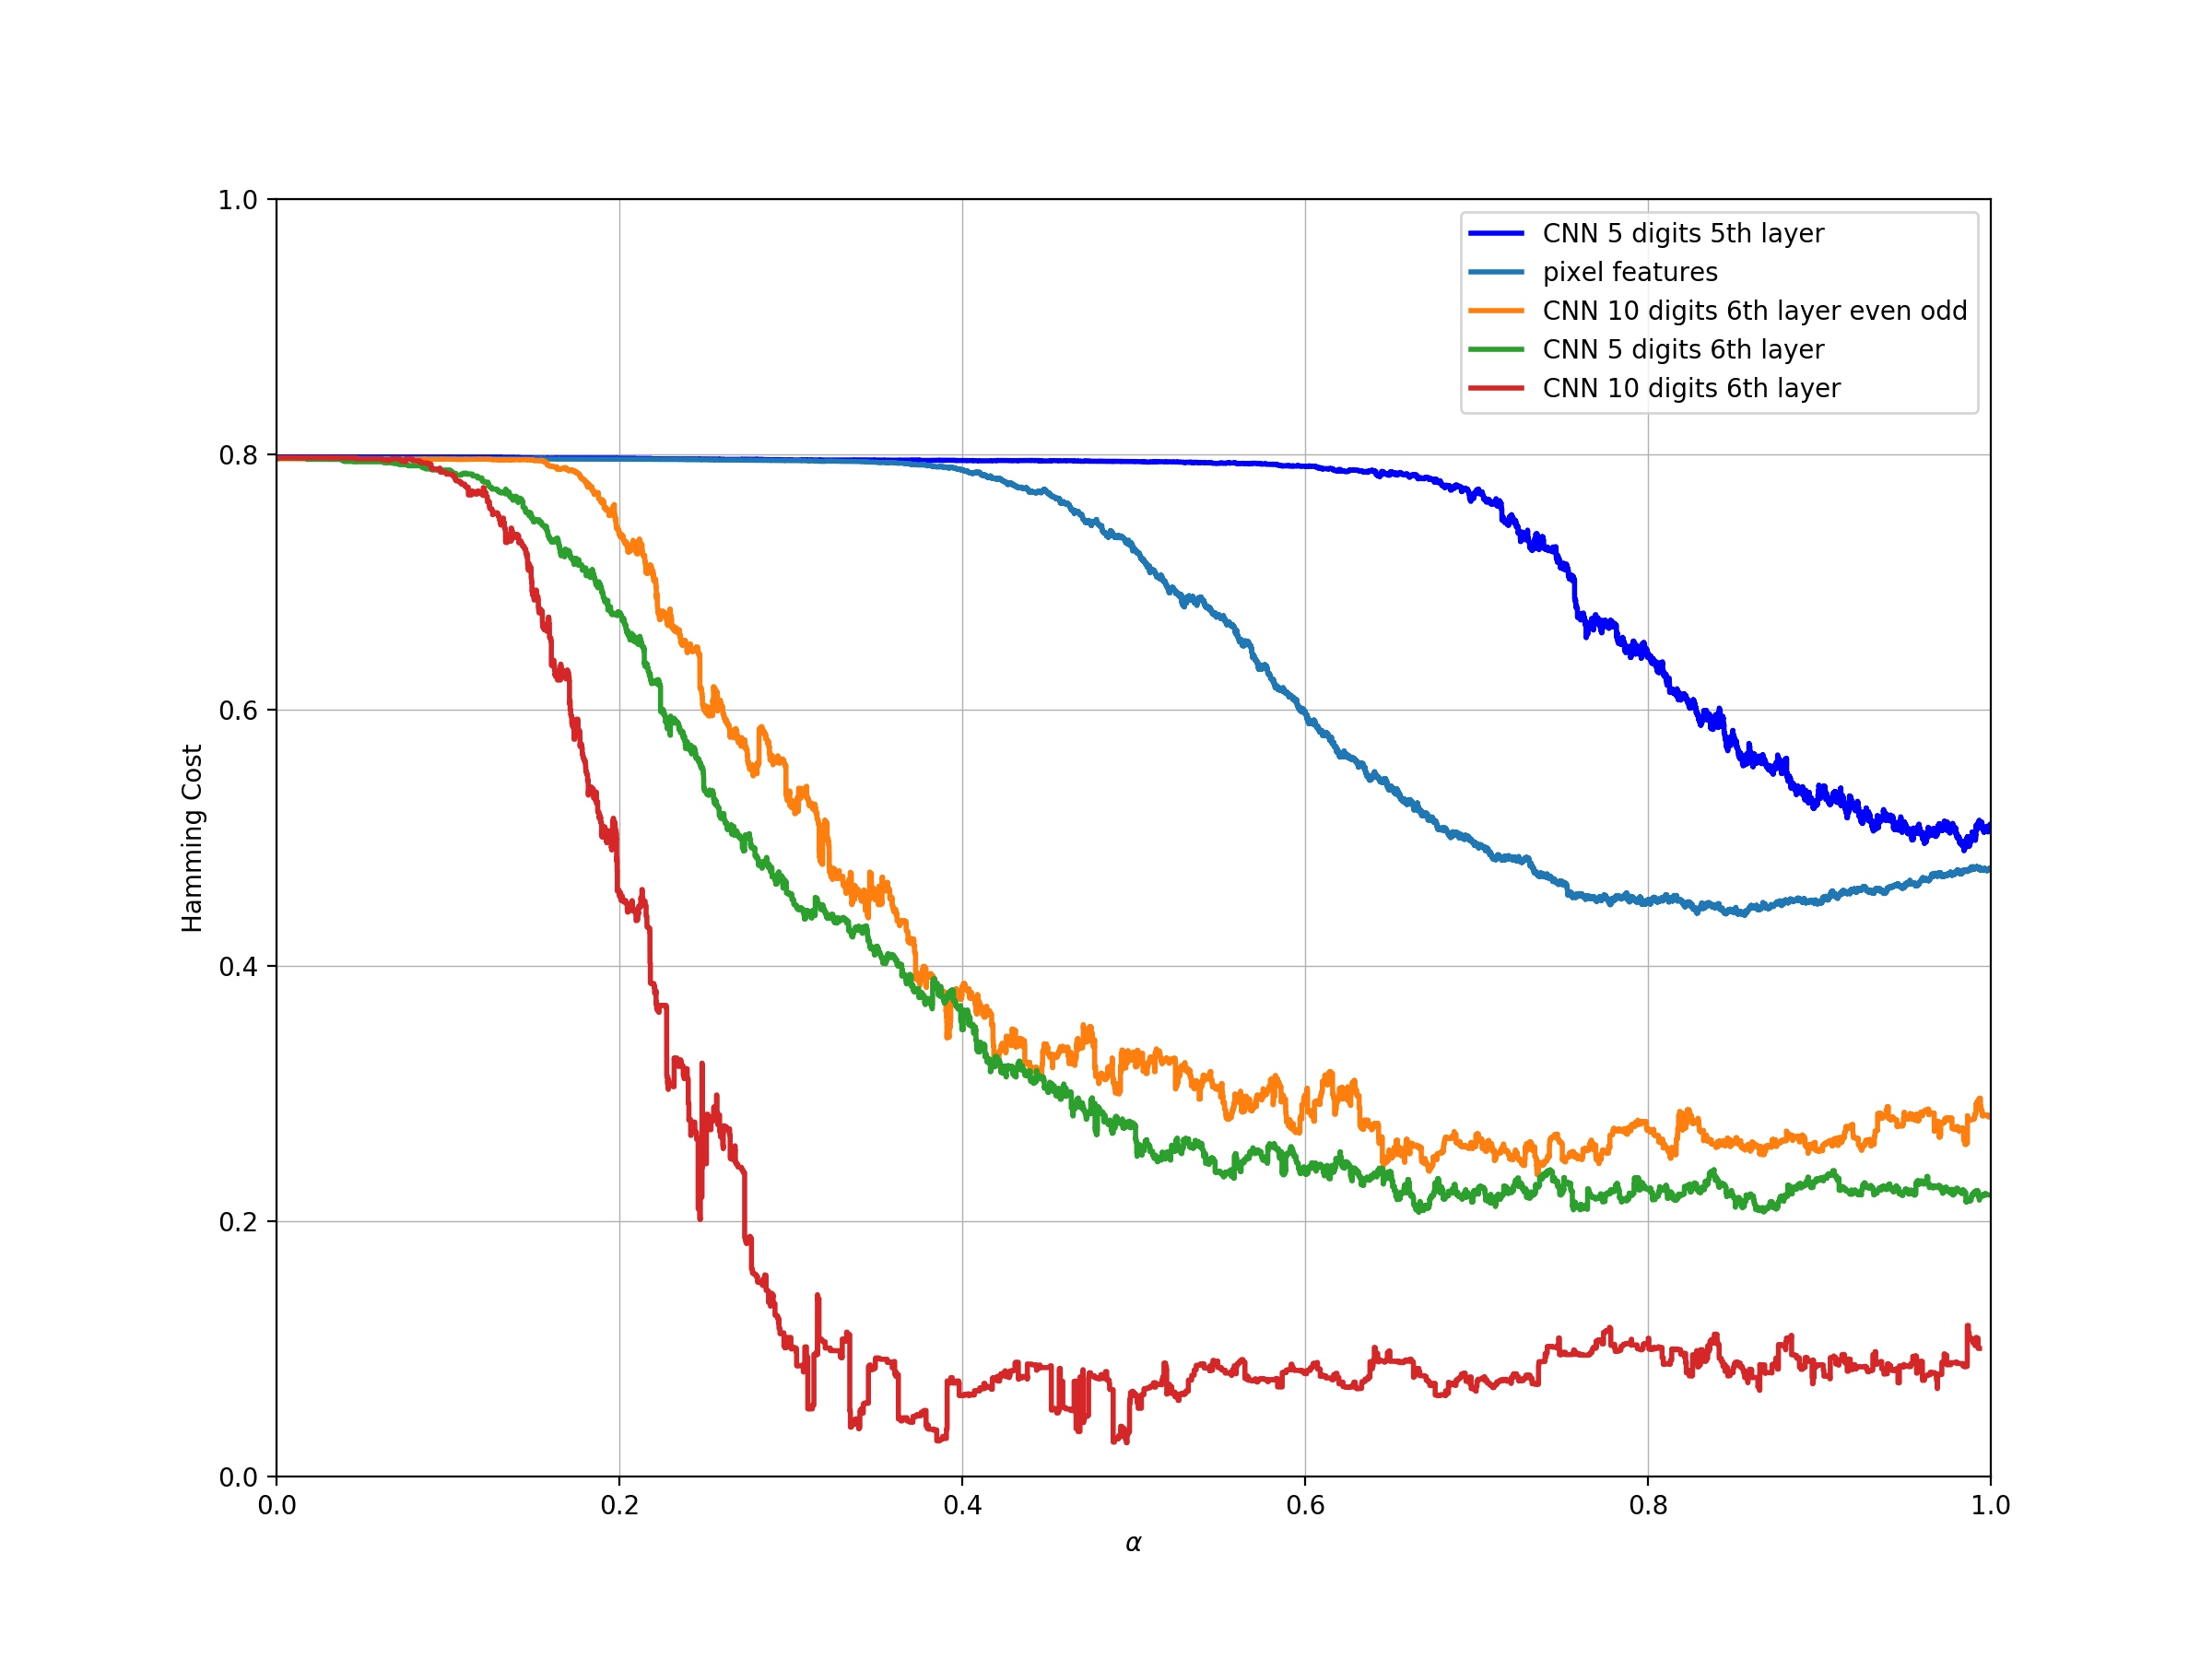
\includegraphics[width=\linewidth]{plots/mnist_overview}}
\end{minipage}\quad
\begin{minipage}{.45\textwidth}
  \centering
  \subcaptionbox{Evaluating 512 experiments with randomized digits and points shows similar results with smoother curves.}
  {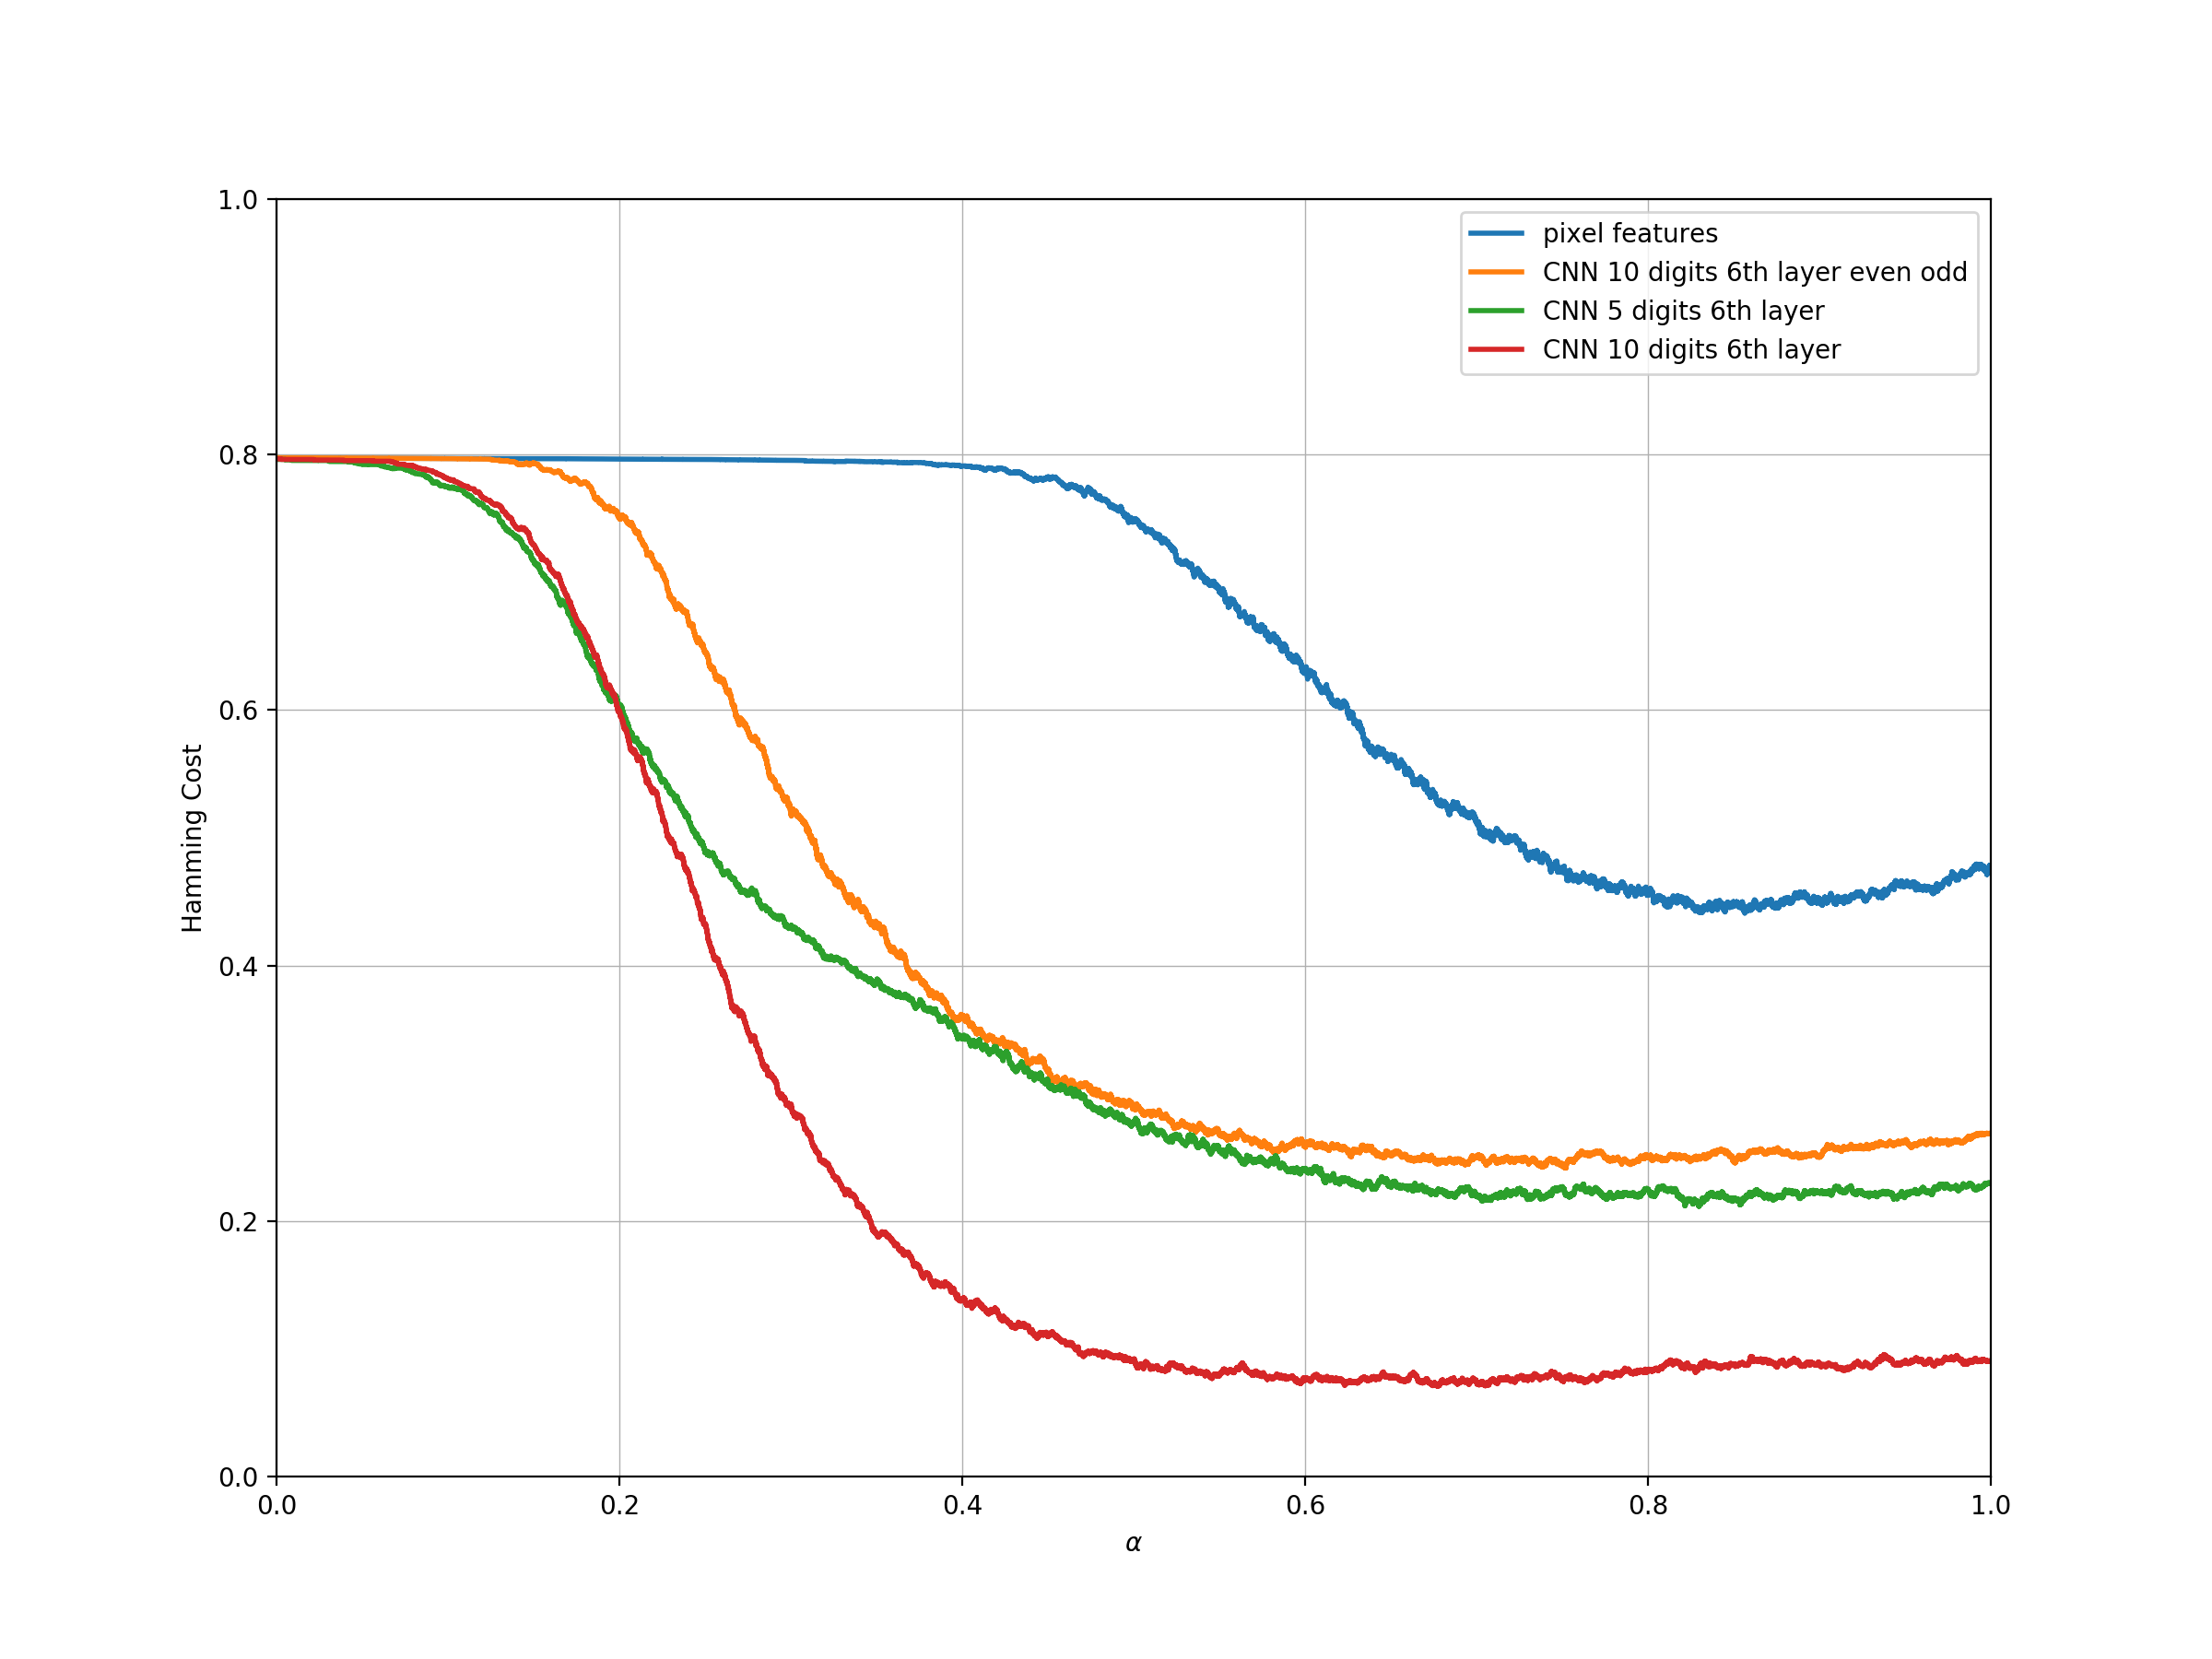
\includegraphics[width=\linewidth]{plots/mnist_overview_random}}
\end{minipage}
\caption{%
  %
  The previously discussed experiments led to different results. While using the features extracted from the fifth layer of the neural network did not lead to good results, features extracted from the sixth layer led to huge improvements.}
  %
\label{fig:mnist_overview}
\end{figure}

\subsection{Omniglot}

The creators of the Omniglot dataset have recently published a review about current results with supervised methods \cite{DBLP:journals/corr/abs-1902-03477}. As this work is only about unsupervised learning, our intention is not to compete with state-of-the-art supervised methods, but rather to outperform common clustering techniques within the following experiments.

\paragraph{Intra-Alphabet Experiments.} The Omniglot dataset contains 30 different alphabets. We cluster all alphabets independently and average over all clustering instances. To see the results for specific alphabets, please see appendix \ref{app:omniglot}. In this section we average the results over all alphabets for $\dsc$ and $\dac$. Figure \ref{fig:omniglot_overview} shows that in both settings complete linkage performs best and our empirical results are slightly better than it. Interpolating between single and complete linkage leads to an error of $71.5\%$ for complete linkage while the optimal parameter $\alpha = 0.908$ leads to an error of $70.5\%$ that makes an improvement of $1.0\%$. When interpolating between average and complete linkage, $\alpha_{opt} = 0.798$ results again in an error of $70.5\%$ that makes the  same improvement of $1.0\%$. We notice that even with the slight improvements we obtain, the error is still very high. This may be caused by the large number of classes (up to 22 in certain alphabets) used in the Omniglot dataset, where a random guess will result in an error of up to $\approx 95.5\%$ depending on the selected alphabet. Again, we observe that single linkage does not perform well at all, however complete linkage leads to significant improvements over a random guess.

\paragraph{CNN Features.} In addition to clustering the raw pixels, we also use the previously discussed CNN architecture trained on all MNIST images to create a better feature representation. We again cluster all alphabets separately, where we show the results for all alphabets in appendix \ref{app:omniglot}. Figure \ref{fig:omniglot_overview} shows that the feature representations lower the error a lot. When interpolating between single and complete linkage, we note that single linkage does not perform better with the new features. However, complete linkage leads to an error of $61.0\%$ that is an improvement of $10.5\%$ over the raw pixels. In addition for $\alpha_{opt} = 0.835$, the error is $59.6\%$, i.e.\ an improvement of $1.4\%$ over complete linkage. When interpolating between average and complete linkage, $\alpha_{opt} = 0.435$ reduces the cost by $2.1\%$ to $58.9\%$.

\paragraph{Inter-Alphabet Experiments.} In addition, we try to cluster characters taken from different alphabets. In our setting, we select one character from each alphabet randomly and run multiple repetitions of this setting where each run contains 30 classes, i.e. 600 points. One advantage of this setting is that each run has the same amount of target clusters that makes it easier to average the results over all experiments. Figure \ref{fig:omniglot_overview} shows that also for clustering characters of different alphabets the improvements are rather small. Averaged over 250 runs the improvement shown below is $1.0\%$.

\begin{figure}[H]
  \centering
  \begin{minipage}{.45\textwidth}
  \centering
  \subcaptionbox{By running experiments within individual alphabets (intra-alphabet), we obtain major improvements over complete linkage for different strategies.}
  {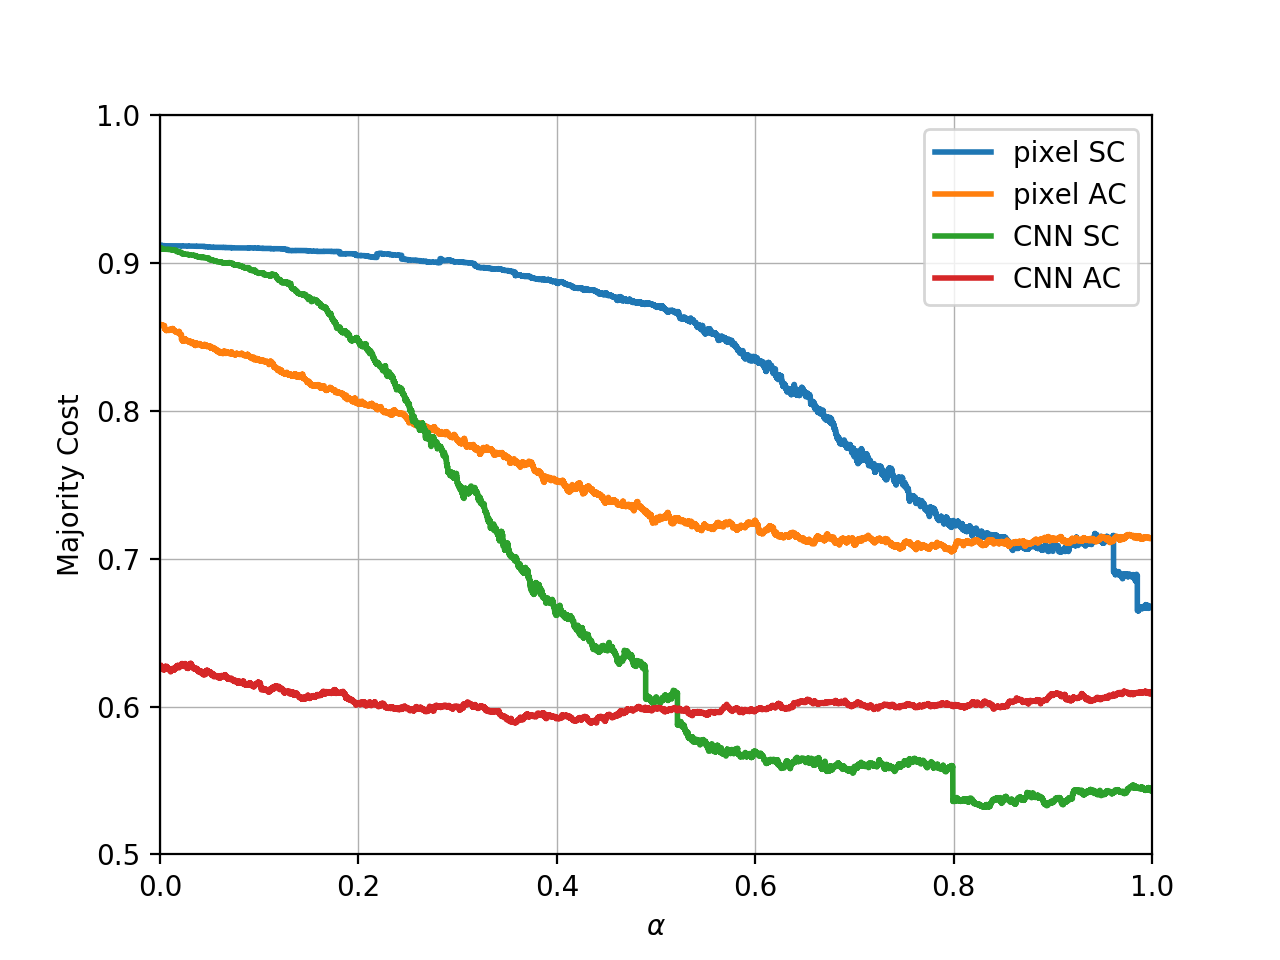
\includegraphics[width=\linewidth]{plots/omniglot_all}}
\end{minipage}\quad
\begin{minipage}{.45\textwidth}
  \centering
  \subcaptionbox{$\alpha$-linkage again leads to noticeable improvements when clustering characters combined from different alphabets (inter-alphabet).}
  {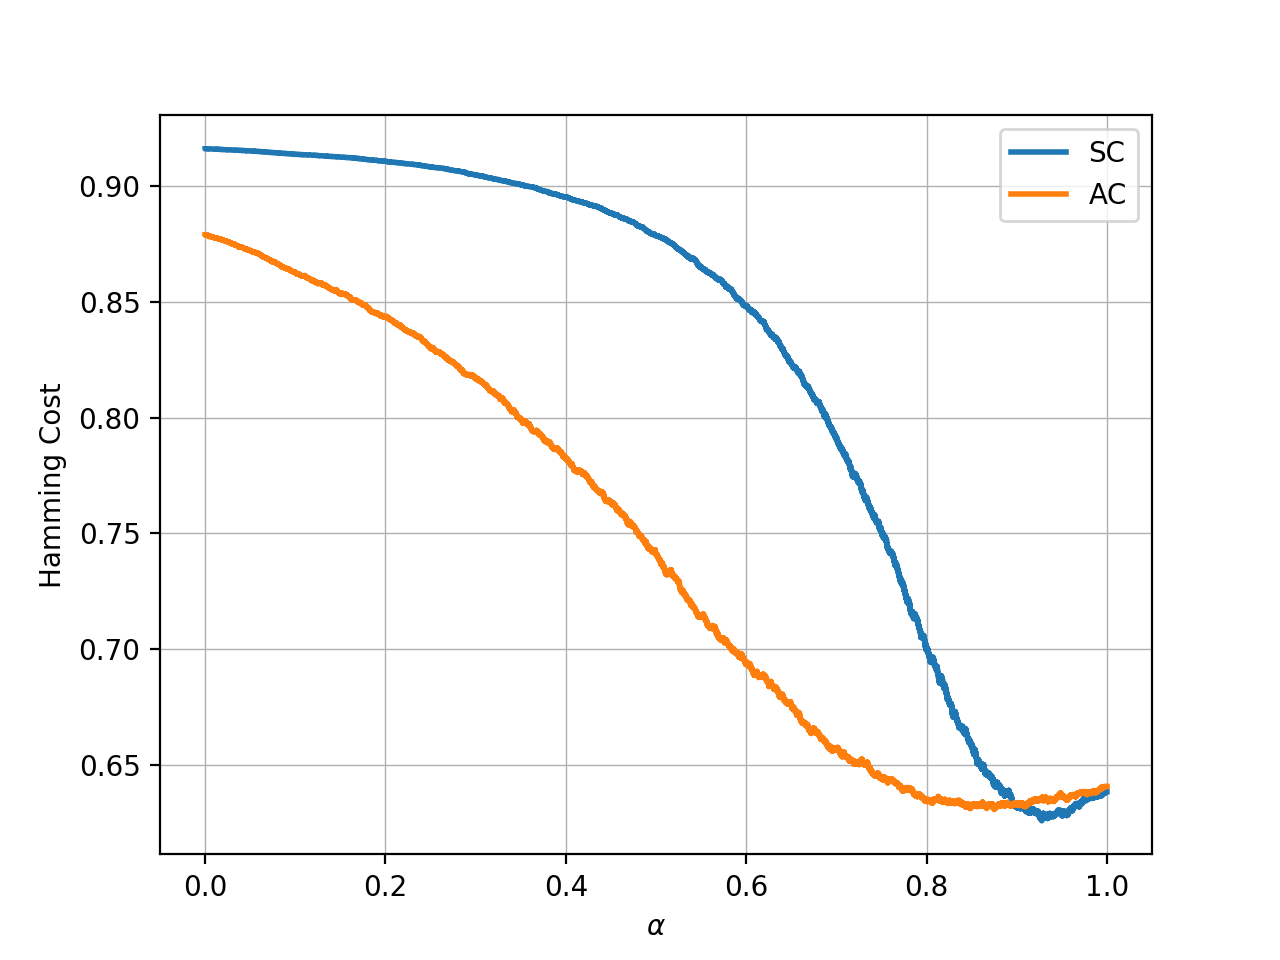
\includegraphics[width=\linewidth]{plots/omniglot_inter}}
\end{minipage}
\caption{For the Omniglot data, we evaluate pixel features for interpolating within each individual alphabet (a) and across different alphabets (b). Also, we evaluate CNN features of a network trained on the MNIST data that lead to major improvements in the intra-alphabet setting (a).}
\label{fig:omniglot_overview}
\end{figure}

\subsection{CIFAR-10}

For the CIFAR-10 data, we only have 10 different classes, so we can only cluster these classes. In the first setting, we cluster all different combinations of five different labels and later average the results over all 252 experiments. Figure \ref{fig:cifar10res} (a) shows the results when interpolating between single and complete linkage. While complete linkage has an error of $51.3\%$, the optimal parameter $\alpha = 0.917$ when interpolating between single and complete linkage improves the clustering by $0.2\%$. As this is only a very small improvement, we decided not to proceed with this dataset and focus on the CIFAR-100 dataset instead that allows a bigger variety of experiments.

\begin{figure}[H]
  \centering
  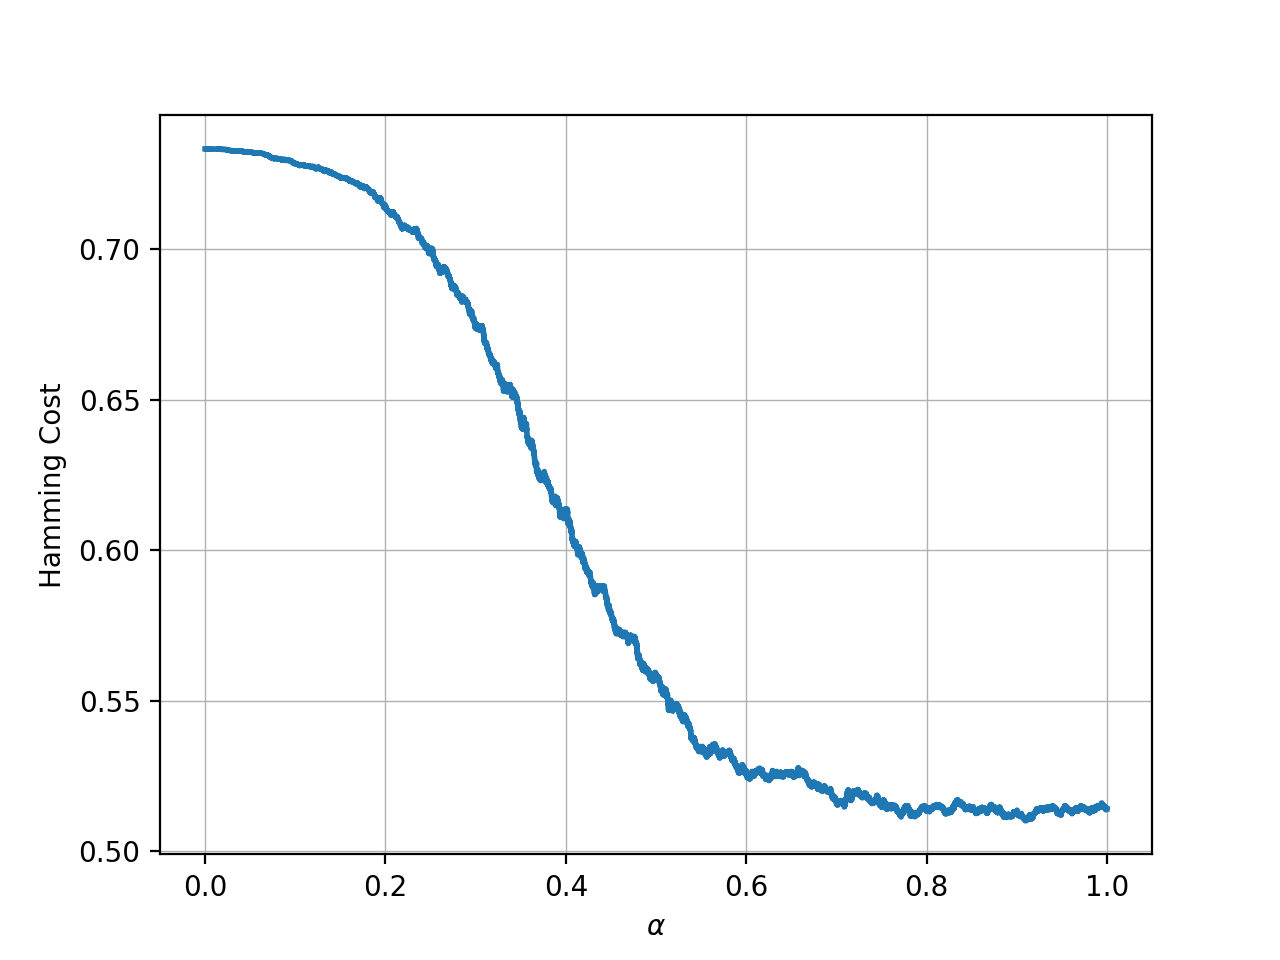
\includegraphics[width=.6\textwidth]{plots/cifar10_sc}
  \caption{Experiments for the CIFAR-10 dataset do not lead to significant improvements.}
  \label{fig:cifar10res}
\end{figure}

\subsection{CIFAR-100}

The CIFAR-100 dataset contains 20 high-level classes, e.g.\ insects and trees, and five low-level classes for each high-level class, e.g. $\{$bee, cockroach$\} \in$ insects and $\{$oak, palm$\} \in$ trees. In the following experiments, we denote the high-level classes as superclasses and the low-level classes as subclasses.

\paragraph{Inter-Superclass Experiments.} We try to cluster as diverse as possible superclasses of the CIFAR 100 dataset by manually picking the five superclasses fish, flowers, household furniture, people and vehicles 1. For each superclass we pick one subclass randomly and evaluate the results for the different combinations of subclasses. In addition to the experiments with $k = 5$ clusters, we compare these results to the results for picking two different subclasses of each superclass resulting in $k = 10$ clusters and also for picking three different subclasses resulting in $k = 15$ clusters, i.e. we combine very diverse and very similar subclasses.

\paragraph{Intra-Superclass Experiments.} In comparison to picking as diverse as possible superclasses, we also evaluate the performance for as similar as possible subclasses. Similar subclasses are already given in the dataset through the subclasses within one superclass. We then evaluate the Hamming cost for each superclass and average the costs over all 20 superclasses to find an optimal value for the parameter $\alpha$. 

\paragraph{Results.} Figure \ref{fig:cifar100} shows the results for the different experiments. We observe that clustering diverse classes in general leads to a lower error than clustering similar images. While for the intra-superclass experiments, complete linkage results in an error of $66.5\%$, it is $61.3\%$ for inter-superclass experiments with images from the manually drawn superclasses. When interpolating between average and complete linkage, $\alpha$-linkag reduces the error in the intra setting by $1.8\%$ for $\alpha = 0.875$ leading to $64.7\%$ and by $0.5\%$ for $\alpha = 0.821$ leading to an error of $60.8\%$. For using $k = 10$ and $k = 15$ clusters, we observe less significant improvements.

\begin{figure}[H]
  \centering
  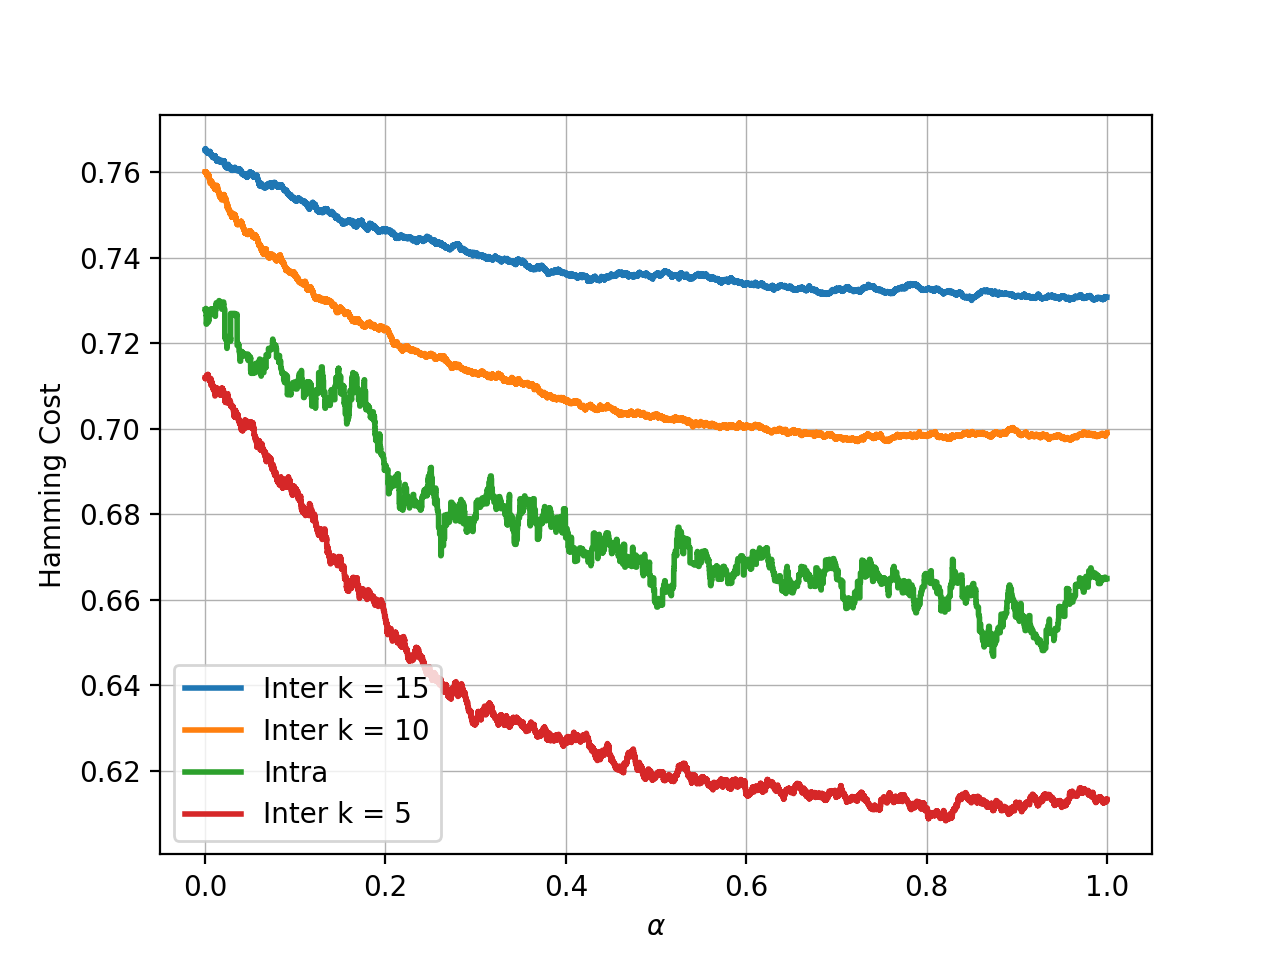
\includegraphics[width=.6\textwidth]{plots/cifar100}
  \caption{Clustering diverse samples of the CIFAR-100 datasets leads to better results than clustering similar images.}
  \label{fig:cifar100}
\end{figure}

We summarize that in general it is easier to cluster rather diverse classes of images, however when clustering more similar images, i.e.\ for more difficult learning tasks, $\alpha$-linkage leads to more significant improvements.

\section{Metric Learning}
\label{sec:metric}

In this section, we apply the introduced framework to learning metrics as suggested in section \ref{sec:beta}. Therefore, we use the Omniglot dataset and evaluate two different settings.

\paragraph{Fixed Amount of Classes.} In the first setting, we follow \cite{NIPS2016_6385} and \cite{pmlr-v70-finn17a}, select $k = 5$ random characters across different alphabets and take the 20 examples of those five characters resulting in a dataset with $n = 100$ examples.

\paragraph{Varying Amount of Classes.} Here, we follow \cite{DBLP:journals/corr/abs-1903-03096} and generate a random number for the amount of $k$ classes between $5$ and $10$. Here, we select the $k$ characters from one randomly selected alphabet, i.e.\ each experiment clusters characters taken from a random alphabet. We again use all $20$ examples for each character.

\paragraph{Distance Metrics.} We present results for mixing three different distance metrics on the Omniglot data. This dataset provides two different representations for each example: a $105 \times 105$ black and white image of the character, and stroke data describing the path that the pen took when writing that character (i.e. a time series of $(x,y)$ coordinates). We use a hand-designed distance metric based on the stroke data, as well as features derived from a Convolutional Neural Network trained on MNIST.
%
\begin{itemize}
  %
  \item (Stroke distance) Given two pen stroke trajectories $s = (x_t,
  y_t)_{t=1}^T$ and $s' = (x'_t, y'_t)_{t=1}^T$, we define the distance between
  them by
  %
  \[
    d(s,s') = \frac{1}{T + T'} \left(
      \sum_{t=1}^T d\bigl((x_t, y_t), s'\bigr)
      +
      \sum_{t=1}^{T'} d\bigl((x'_t, y'_t), s\bigr)
    \right),
  \]
  %
  where $d\bigl((x_t, y_t), s'\bigr)$ denotes the Euclidean distance from the
  point $(x_t, y_t)$ to the closest point in $s'$. This is the average distance
  from any point from either trajectory to the nearest point on the other
  trajectory.
  %
  \item (CNN-C) Next we construct a distance metric using the image
  representation of each example. In particular, we train a Convolutional Neural
  Network for classifying the 10 digits of MNIST. Then we use this network to
  obtain embeddings of each omniglot digit. Finally, to measure the distance
  between two examples, we use the cosine distance between them, i.e.\ the
  angle between the two feature embeddings.
  %
  \item (CNN-E) The final metric uses the same neural network embedding as
  above, except measures distances between two examples using the Euclidean
  distance.
  %
\end{itemize}

\paragraph{Results.} Figure \ref{fig:dl-omniglot} shows our empirical results for learning the best combinations of the above metrics on both instance
distributions over the Omniglot dataset. For each pair of metrics and each
instance distribution, we plot the average Hamming error of the cluster tree
produced by the algorithm as a function of the mixing parameter $\beta$ averaged
over $N = 2000$ clustering instances sampled from the underlying distribution.
For both distributions, the best mixture of two metrics performs better than the
best fixed single metric. On the distribution with $k=5$ clusters, the best average
performance is obtained when mixing the Euclidean and cosine distances for the
MNIST CNN features with $\beta = 0.727$ achieving an average Hamming error of
$26.3\%$. In contrast, using the cosine distance on the MNIST CNN features is the
best single metric and has an average Hamming error of $28.9\%$, yielding an
improvement of $2.6\%$. For the instance distribution with a variable amount of classes, the stroke distance
appears to be more useful. The best performance is achieved when mixing the
stroke distance and the cosine distance on the MNIST CNN features with $\beta =
0.514$ and achieves an error of $33\%$, while the best fixed metric has an error of $42\%$,
leading to an improvement of $9\%$.


\begin{figure}[H]
  \begin{subfigure}[b]{0.5\textwidth}
    \centering
    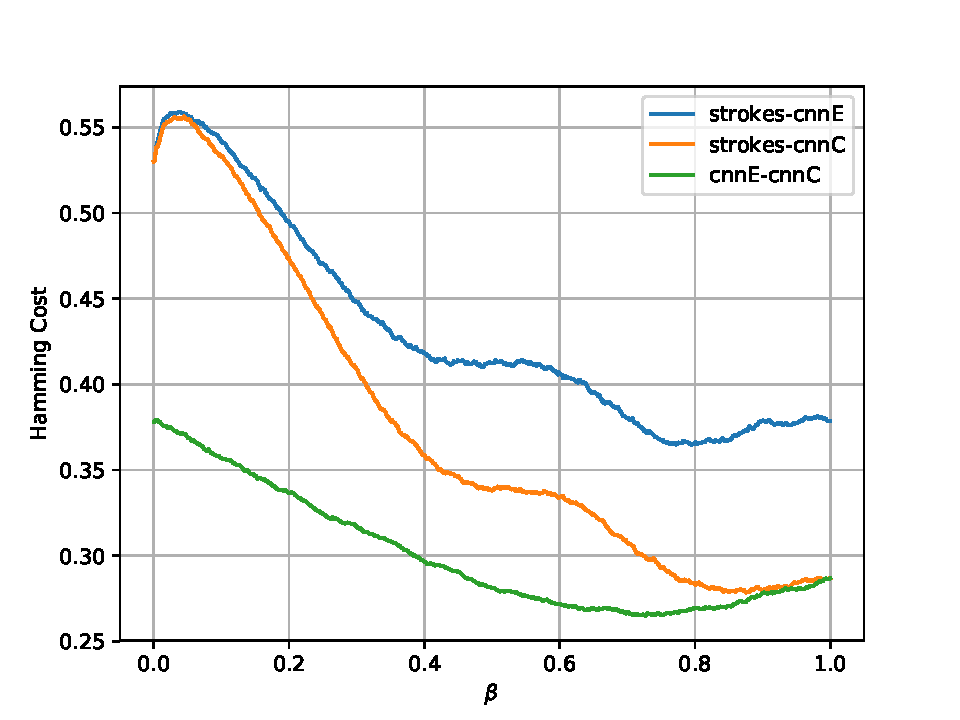
\includegraphics[width=0.9\textwidth]{plots/omniglot_MAML_results}
    \caption{Choosing $k=5$ different characters from different alphabets improves the cost by $2.6\%$ when combining the Euclidean and the cosine distance of the MNIST CNN features.}
    \label{fig:dl-omniglot-maml}
  \end{subfigure}\quad
  ~
  \begin{subfigure}[b]{0.5\textwidth}
    \centering
    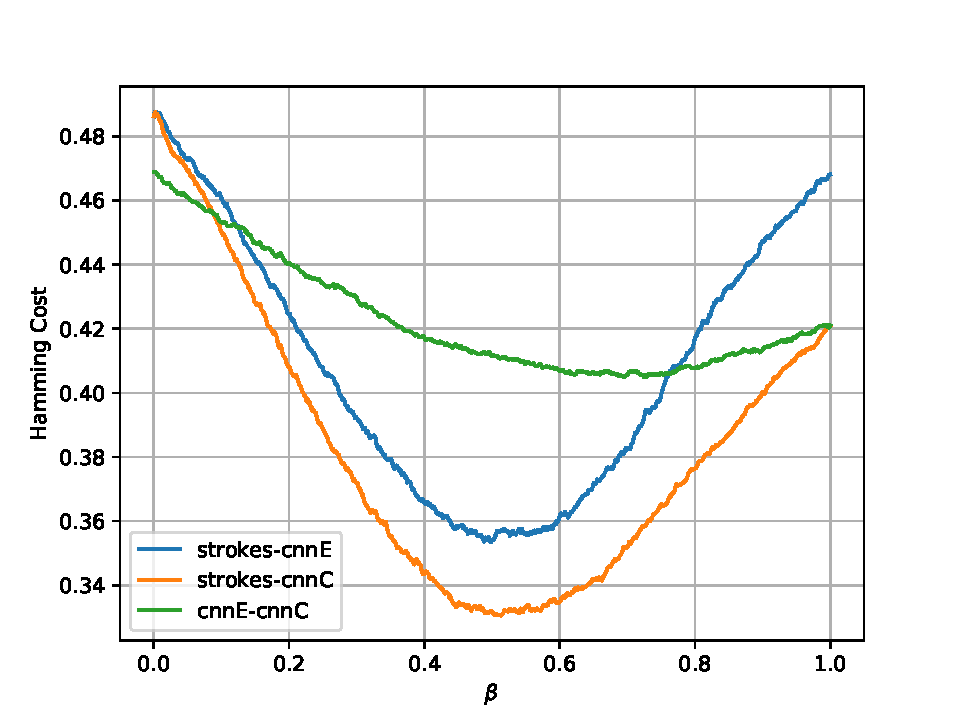
\includegraphics[width=0.9\textwidth]{plots/omniglot_MD2_results}
    \caption{Selecting $k$ between $5$ and $10$ characters of the same alphabet improves the cost by $9\%$ when combining the stroke features and the cosine distance of the MNIST CNN features.}
    \label{fig:dl-omniglot-md}
  \end{subfigure}
  \caption{Learning the best distance metric for Omniglot leads to improvements of up to $9\%$ when combining the time series stroke data with the cosine distance of the MNIST CNN features.}
  \label{fig:dl-omniglot}
\end{figure}
